\graphicspath{{chapters/deep_learning/}}

\chapter{Deep Stochastic CCA: Bridging Multiview and Self-Supervised Learning}\label{ch:deep_learning}
\minitoc
% chktex-file 44
% chktex-file 3
\section*{Preface}

This chapter is based on work presented in \citet{chapman2023cca} and \citet{chapman2023efficient}.

\section{Introduction}

Deep CCA \citep{andrew2013deep} secured a runner-up position for the test-of-time award at ICML 2023 \citep{ICML2023TOT}.
However, its direct application has been limited in large datasets due to biased gradients in the stochastic minibatch setting.
There have since been proposals to scale-up Deep CCA in the stochastic case with adaptive whitening \citep{wang2015stochastic} and regularization \citep{chang2018scalable}, but these techniques are highly sensitive to hyperparameter tuning.

Self-Supervised Learning (SSL) methods have reached the state-of-the-art in tasks such as image classification \citep{balestriero2023cookbook}, learning representations without labels that capture salient features so that they can be used for general downstream tasks.
A family of SSL methods that are closely aligned with Canonical Correlation Analysis (CCA) has garnered particular interest.
This family notably includes Barlow Twins \citep{zbontar2021barlow}, VICReg \citep{bardes2021vicreg}, and W-MSE \citep{ermolov2021whitening} and they aim to transform a pair of data views into similar representations, similar to the objective of CCA. Similarly, some generative approaches to SSL\citep{sansone2022gedi} bear a striking resemblance to Probabilistic CCA\citep{bach2005probabilistic}.
These connections have started to be explored in \citet{balestriero2022contrastive}.

In this chapter, we propose a novel formulation of Deep CCA that is unbiased in the stochastic setting and scales to large datasets.
We also propose a novel SSL method, SSL-EY, that is competitive with existing methods on CIFAR-10 and CIFAR-100.
We highlight the connections between our work and existing SSL methods, and show that our method is more robust to hyperparameter tuning.

\section{Background: Deep Representation Learning}

This section explores the evolution of deep representation learning techniques, from traditional autoencoders to more sophisticated approaches like Deep Canonical Correlation Analysis (Deep CCA) and Self-Supervised Learning (SSL).

\subsection{Deep Learning and Neural Networks}
Deep learning, a subfield of machine learning, utilizes neural networks to learn complex representations from data. Neural networks are composed of interconnected layers of artificial neurons, typically including an input layer, one or more hidden layers, and an output layer. Each neuron computes a weighted sum of its inputs, followed by a nonlinear activation function.
A key component of modern neural networks is the rectified linear unit (ReLU) activation function, defined as:
\begin{equation}
\ReLU(x) = \max(0, x)
\end{equation}
ReLU and its variants have become popular due to their simplicity and effectiveness in mitigating the vanishing gradient problem during training.
The power of neural networks lies in their ability to approximate complex functions. The Universal Approximation Theorem \citep{cybenko1989approximation,hornik1991approximation} states that a feedforward network with a single hidden layer containing a finite number of neurons can approximate any continuous function on compact subsets of $\mathbb{R}^n$, given certain mild assumptions about the activation function.
Neural networks are typically trained using backpropagation and stochastic gradient descent (SGD) or its variants. The backpropagation algorithm efficiently computes gradients of the loss function with respect to the network parameters, while SGD allows for training on large datasets by updating parameters using small batches of data.
\subsection{Autoencoders and Representation Learning}
Autoencoders represent an early approach to unsupervised representation learning. These neural networks are designed to learn compact data representations by reconstructing input data through a bottleneck layer. The basic structure of an autoencoder consists of:

An encoder function $f_{\theta}: \mathcal{X} \to \mathcal{Z}$ that maps input data to a latent representation.
A decoder function $g_{\phi}: \mathcal{Z} \to \mathcal{X}$ that attempts to reconstruct the input from the latent representation.

The autoencoder is trained to minimize a reconstruction loss:
\begin{equation}
\mathcal{L}(\theta, \phi) = \mathbb{E}{x \sim p{\text{data}}}[|x - g_{\phi}(f_{\theta}(x))|^2]
\end{equation}
Autoencoders can be viewed as a nonlinear generalization of Principal Component Analysis (PCA). In fact, a linear autoencoder with a single hidden layer and mean squared error loss is equivalent to PCA when the hidden layer dimension is less than the input dimension.
While autoencoders have been successful in various applications, they face limitations. The focus on reconstruction may lead to learning fine-grained details that are not necessarily useful for downstream tasks, and there's no explicit encouragement for the learned representations to capture meaningful features or disentangled factors of variation.

These limitations have motivated the development of more sophisticated autoencoder variants and alternative representation learning approaches.
\subsection{Variational Autoencoders}
Variational Autoencoders (VAEs) \citep{kingma2013auto} extend the autoencoder framework to learn probabilistic generative models. VAEs model the latent space as a probability distribution, typically a multivariate Gaussian, and are trained to maximize the evidence lower bound (ELBO):
\begin{equation}
\mathcal{L}{ELBO}(\theta, \phi) = \mathbb{E}{q_{\phi}(z|x)}[\log p_{\theta}(x|z)] - D_{KL}(q_{\phi}(z|x) || p(z))
\end{equation}
where $q_{\phi}(z|x)$ is the encoder (or inference) network, $p_{\theta}(x|z)$ is the decoder (or generative) network, and $p(z)$ is a prior distribution over the latent space.
VAEs provide a principled way to generate new samples and perform probabilistic inference, making them useful for both representation learning and generative modeling.

Given the connection between Autoencoders and PCA, it is natural to consider the extension of CCA to the deep learning setting. This leads to the development of Deep CCA, which aims to learn nonlinear representations that are maximally correlated across different views.

\subsection{From Autoencoders to Deep CCA}

The objective of Deep CCA is to maximize the correlation between learned representations of different views:
\begin{align}
\label{eq:DMCCA-def}
\norm{\MCCA_K\left(Z^{(1)}, \ldots, Z^{(I)}\right)}_2
\end{align}
where $Z^{(i)} = f^{(i)}(X^{(i)}; \theta^{(i)})$ are the learned representations for each view.
\begin{figure}
\centering
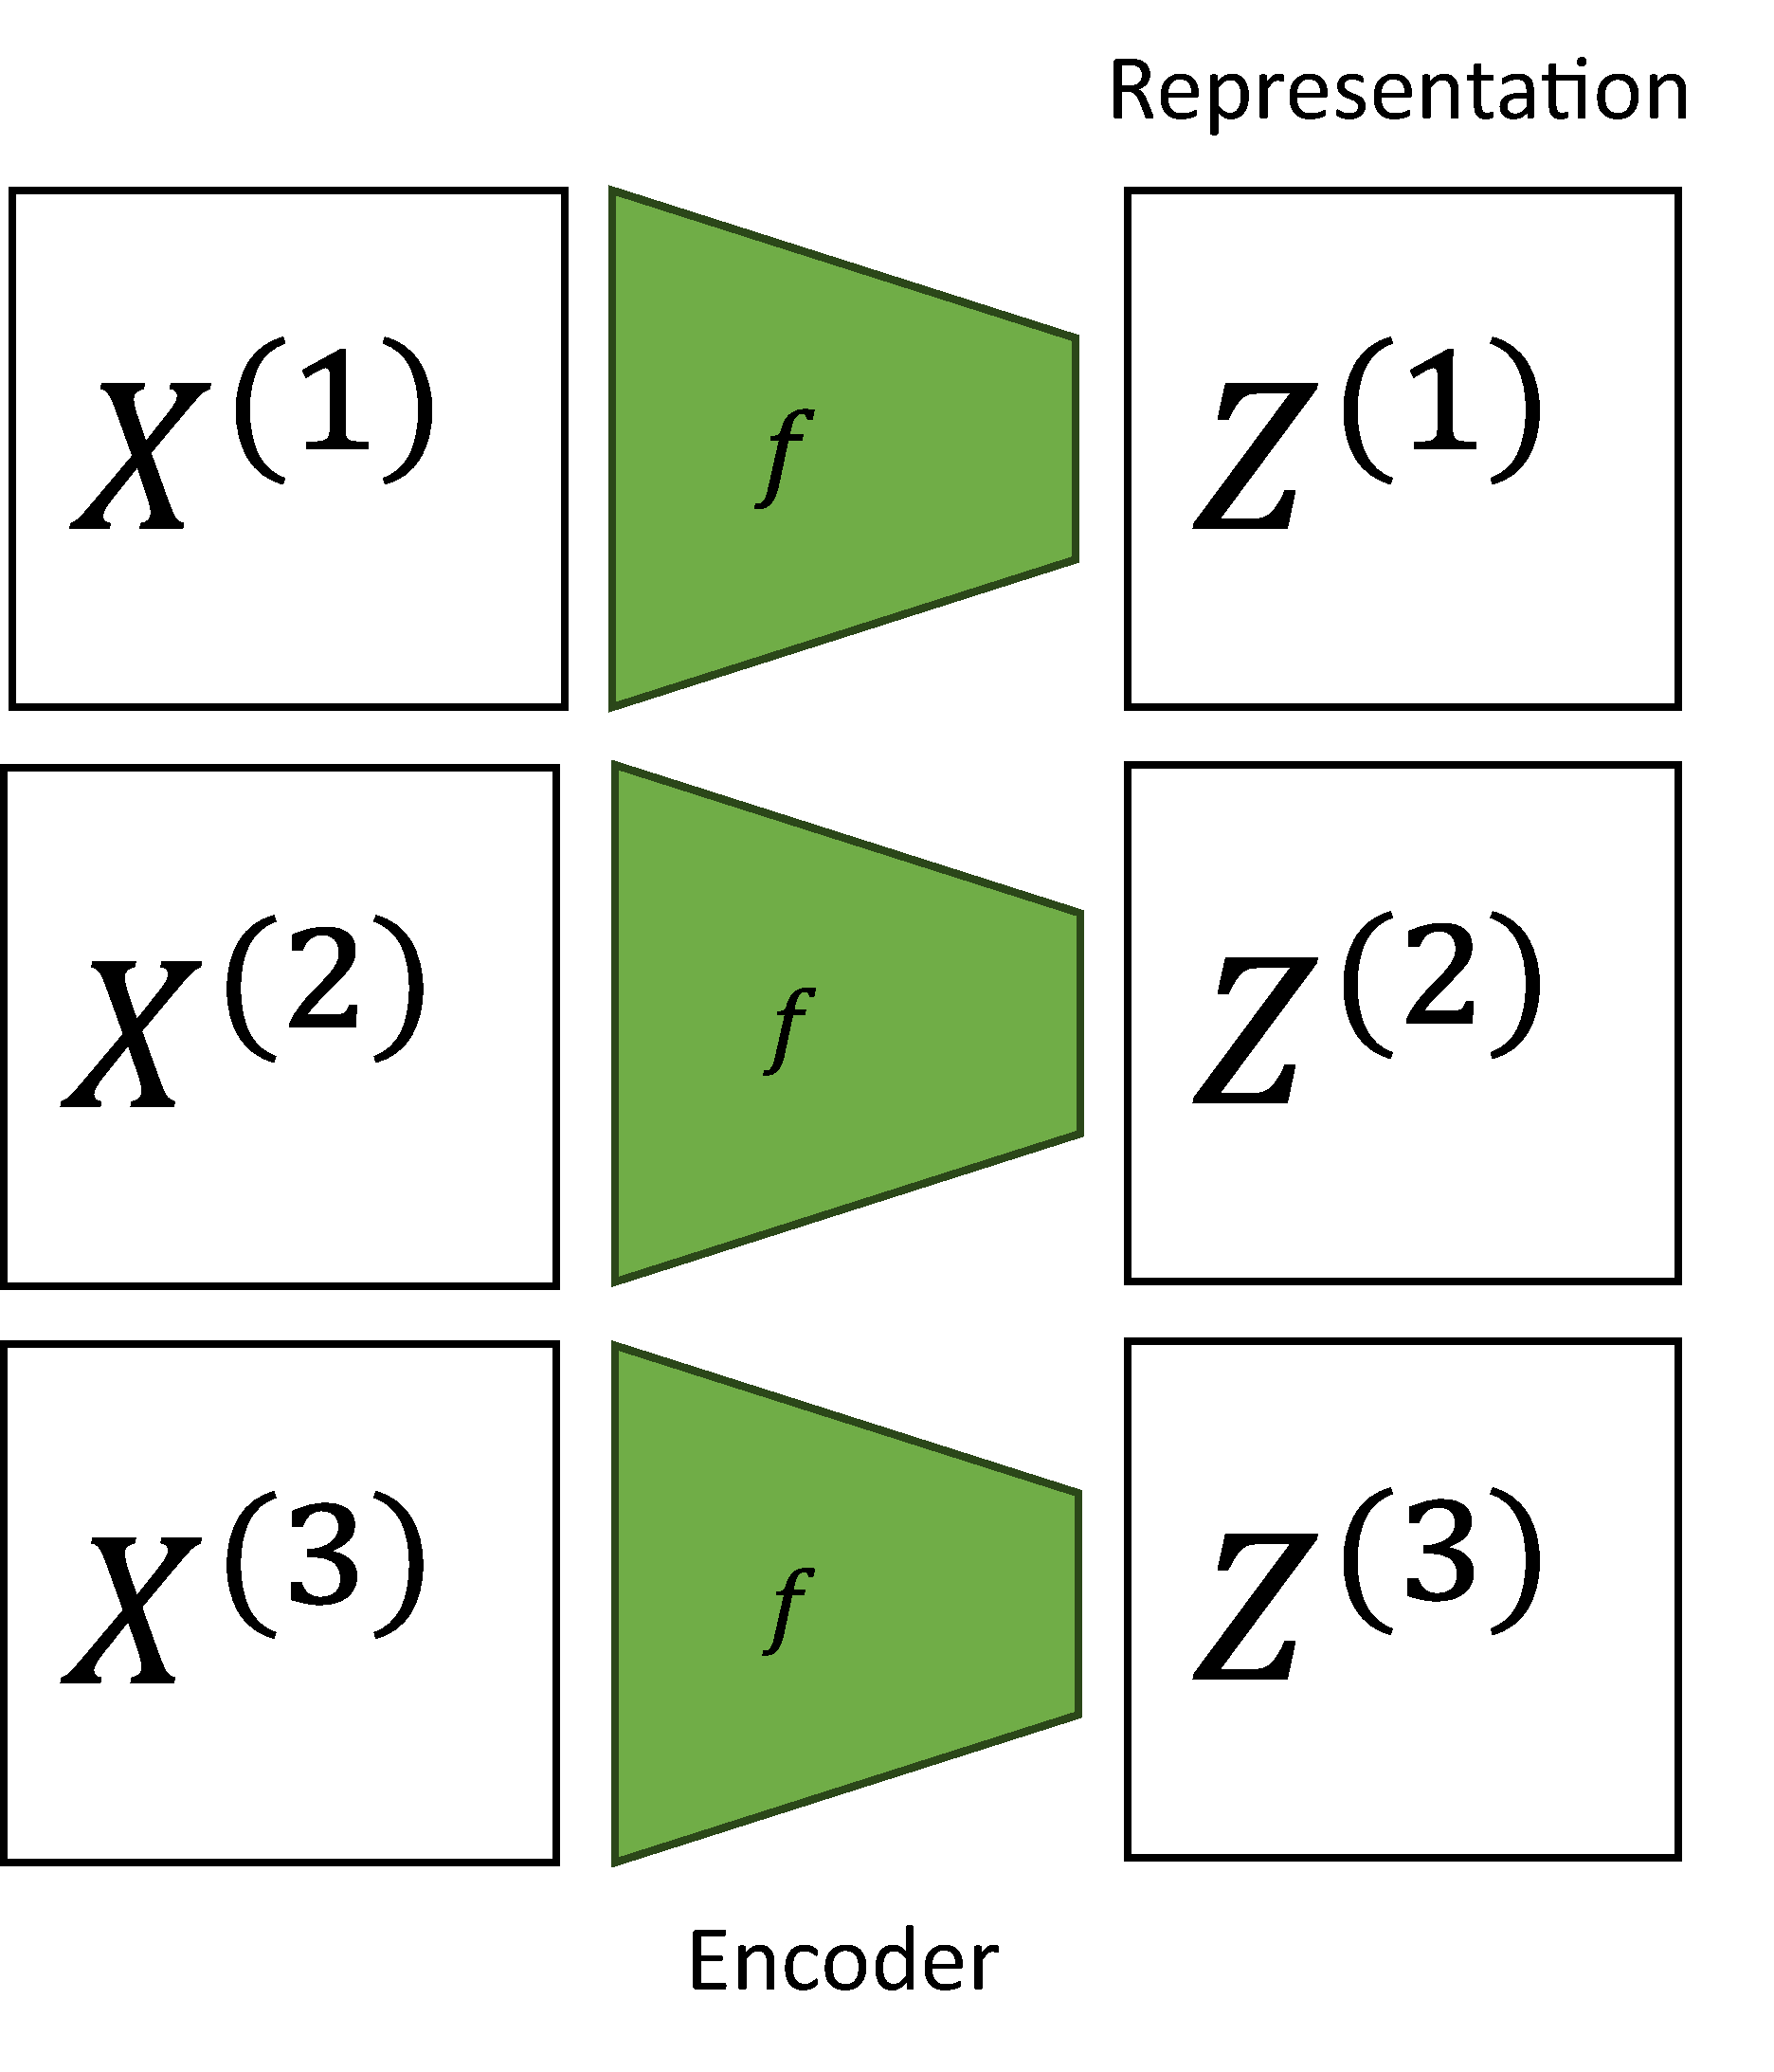
\includegraphics[width=0.5\textwidth]{figures/dcca_schematic}
\caption{Schematic of the Deep CCA approach highlighting the nonlinear transformation of data into correlated views.}
\label{fig:dcca_schematic}
\end{figure}
Figure \ref{fig:dcca_schematic} illustrates how Deep CCA transforms data from different views through neural networks to achieve correlated representations. This approach allows for capturing complex, nonlinear relationships between views that linear methods might miss.

\subsubsection{Full-batch Deep CCA}
The full-batch approach of Deep CCA, formulated by \citet{andrew2013deep}, maximizes correlation using the following loss function:

\begin{align}\label{eq:T_definition}
    T          & = \left(\text{cov}(Z^{(1)})\right)^{-\frac{1}{2}} Z^{(1)\top} Z^{(2)} \left(\text{cov}(Z^{(2)})\right)^{-\frac{1}{2}} \\
    \LRayleigh & = -\Tr(T)
\end{align}

We refer to this as the Rayleigh loss because it effectively maximizes the Generalized Rayleigh Quotient associated with the canonical correlation problem. While theoretically sound, this approach faces significant scalability issues with large datasets.

The Rayleigh loss is only valid for full batch gradient descent, which becomes computationally infeasible for large datasets. This limitation has led to numerous issues reported on the GitHub implementation, with users experiencing problems with ill-conditioned matrices and exploding gradients. These problems arise because the covariance matrices can become singular or nearly singular when working with small batches or high-dimensional data, leading to instability in the matrix inversions required by the loss function.

\subsubsection{DCCA-STOL}
DCCA-STOL, proposed by \citet{wang2015unsupervised}, attempts to use the full-batch objective with large mini-batches but suffers from biased gradients due to the matrix inversions in Equation \eqref{eq:T_definition}. This bias is fundamentally a consequence of Jensen's inequality applied to the inverse of a random variable. 

For a positive random variable $X$, Jensen's inequality states that:

\begin{equation}
\frac{1}{E[X]} \leq E[\frac{1}{X}]
\end{equation}

This inequality arises because $f(x) = \frac{1}{x}$ is a convex function for $x > 0$. 

To illustrate this, consider a simple example: Let $X$ be a random variable that is 1 with probability 0.5 and 0.1 with probability 0.5. Then:

\begin{align}
    E[X] &= 0.5 \cdot 1 + 0.5 \cdot 0.1 = 0.55 \\
    \frac{1}{E[X]} &= \frac{1}{0.55} \approx 1.82 \\
    E[\frac{1}{X}] &= 0.5 \cdot \frac{1}{1} + 0.5 \cdot \frac{1}{0.1} = 0.5 + 5 = 5.5
\end{align}

As we can see, $\frac{1}{E[X]} < E[\frac{1}{X}]$, confirming the inequality. 

In the context of DCCA-STOL, this inequality leads to biased estimates when inverting covariance matrices estimated from mini-batches. The expectation of the inverse of the sample covariance matrix is not equal to the inverse of the expected covariance matrix. This bias necessitates batch sizes larger than the representation size, limiting the method's practical application.

The problem becomes even more severe when the batch size is smaller than the representation dimension. In this case, the sample covariance matrix is guaranteed to be singular. To understand why, consider that a batch of size $n$ in a $d$-dimensional space (where $n < d$) can only span an $n$-dimensional subspace. Consequently, the sample covariance matrix will have at most rank $n$, making it singular in the $d$-dimensional space.

For singular matrices, the inverse is undefined, which is equivalent to division by zero in the scalar case. This causes Jensen's inequality to blow up to infinity, making the optimization problem ill-posed and impossible to solve.

Even when the batch size is slightly larger than the representation dimension, the covariance matrix can be nearly singular, leading to numerical instability and unreliable results.

A practical example illustrates the severity of this issue: Consider training deep neural networks on 3D MRI scans. Due to memory constraints of GPUs, it's often impossible to use large batch sizes for such high-dimensional data. If we attempt to use small batch sizes with the Rayleigh or STOL objective, we encounter singular (when batch size < representation dimension) or near-singular (when batch size $\approx$ representation dimension) matrices. The singularity effectively causes division by zero in Jensen's inequality, blowing up the expectation to infinity.

This problem has caused confusion for many GitHub users (including myself!) who attempted to implement these methods. The nuanced nature of this issue is not immediately apparent, leading to unexpected behavior and optimization failures. It's crucial to understand that to even get the optimization to run, we require batch sizes substantially larger than the representation dimension, before even considering problems of bias. This requirement severely limits the applicability of the method to high-dimensional data or large models, as it demands enormous batch sizes that often exceed available computational resources.

\subsubsection{Deep MCCA and Deep GCCA}
Extensions such as Deep MCCA \citep{somandepalli2019multimodal} and Deep GCCA \citep{benton2017deep} are multiview extensions of Deep CCA. Their loss function is given by:

\begin{align}
    T      & = \left(\hat{V}(\theta)^{-\frac{1}{2}} \hat{C}(\theta)\hat{V}(\theta)^{-\frac{1}{2}}\right) \\
    \LDMCCA & = -\Tr(T)
\end{align}

where $\hat{C}(\theta)$ and $\hat{V}(\theta)$ are the mini-batch estimates of the between-view and within-view covariance matrices. However, these methods still require large batch sizes due to biased gradients from small mini-batch covariance matrices. This issue stems from the same problem as DCCA-STOL: the matrix inversions in the loss function lead to biased estimates when using small mini-batches, again due to Jensen's inequality.

\subsubsection{Adaptive Whitening Methods}
Adaptive whitening methods \citep{wang2015stochastic, chang2018scalable} offer another solution to the scalability problem. These methods aim to approximate the matrix inversion in the loss function without actually inverting the matrix, functioning similarly to a preconditioner in optimization. By doing so, they attempt to mitigate the bias introduced by direct matrix inversion on small mini-batches.

One such method is DCCA-NOI \citep{wang2015unsupervised}, which uses Nonlinear Orthogonal Iteration to approximate the whitening transformation. The loss function of DCCA-NOI is:

\begin{align}
    \LNOI & = |{\tilde{\Sigma}_{11}}^{-\frac{1}{2}} Z\sps{1}-{\tilde{\Sigma}_{22}}^{-\frac{1}{2}} Z\sps{2}|^2_F
\end{align}

where $\tilde{\Sigma}_{11}$ and $\tilde{\Sigma}_{22}$ are estimates of the covariance matrices of $Z\sps{1}$ and $Z\sps{2}$. The adaptive whitening approach aims to iteratively refine these estimates over time, potentially allowing for smaller batch sizes. However, these methods introduce a time constant that complicates analysis and requires extensive tuning. This time constant represents the rate at which the whitening estimates are updated, and finding the right balance between stability and adaptivity can be challenging.

\subsection{Self-Supervised Learning and Joint Embedding}

Self-Supervised Learning (SSL) has emerged as a powerful approach for learning representations from unlabeled data. A key strategy in SSL involves creating joint embeddings of augmented data, typically images.

\begin{figure}
\centering
\tikz{
    \node[latent, align=center] (x) {Original Data\\$X$};
    \node[obs, below left=of x, align=center] (x1) {Augmented Data\\$X^{(1)}$};
    \node[obs, below right=of x, align=center] (x2) {Augmented Data\\$X^{(2)}$};
    \edge{x} {x1}
    \edge{x} {x2}
}
\caption{Joint Embedding Data Generation Process in SSL}
\label{fig:joint_embedding}
\end{figure}

SSL methods often employ an encoder-projector model:

\begin{figure}
\centering
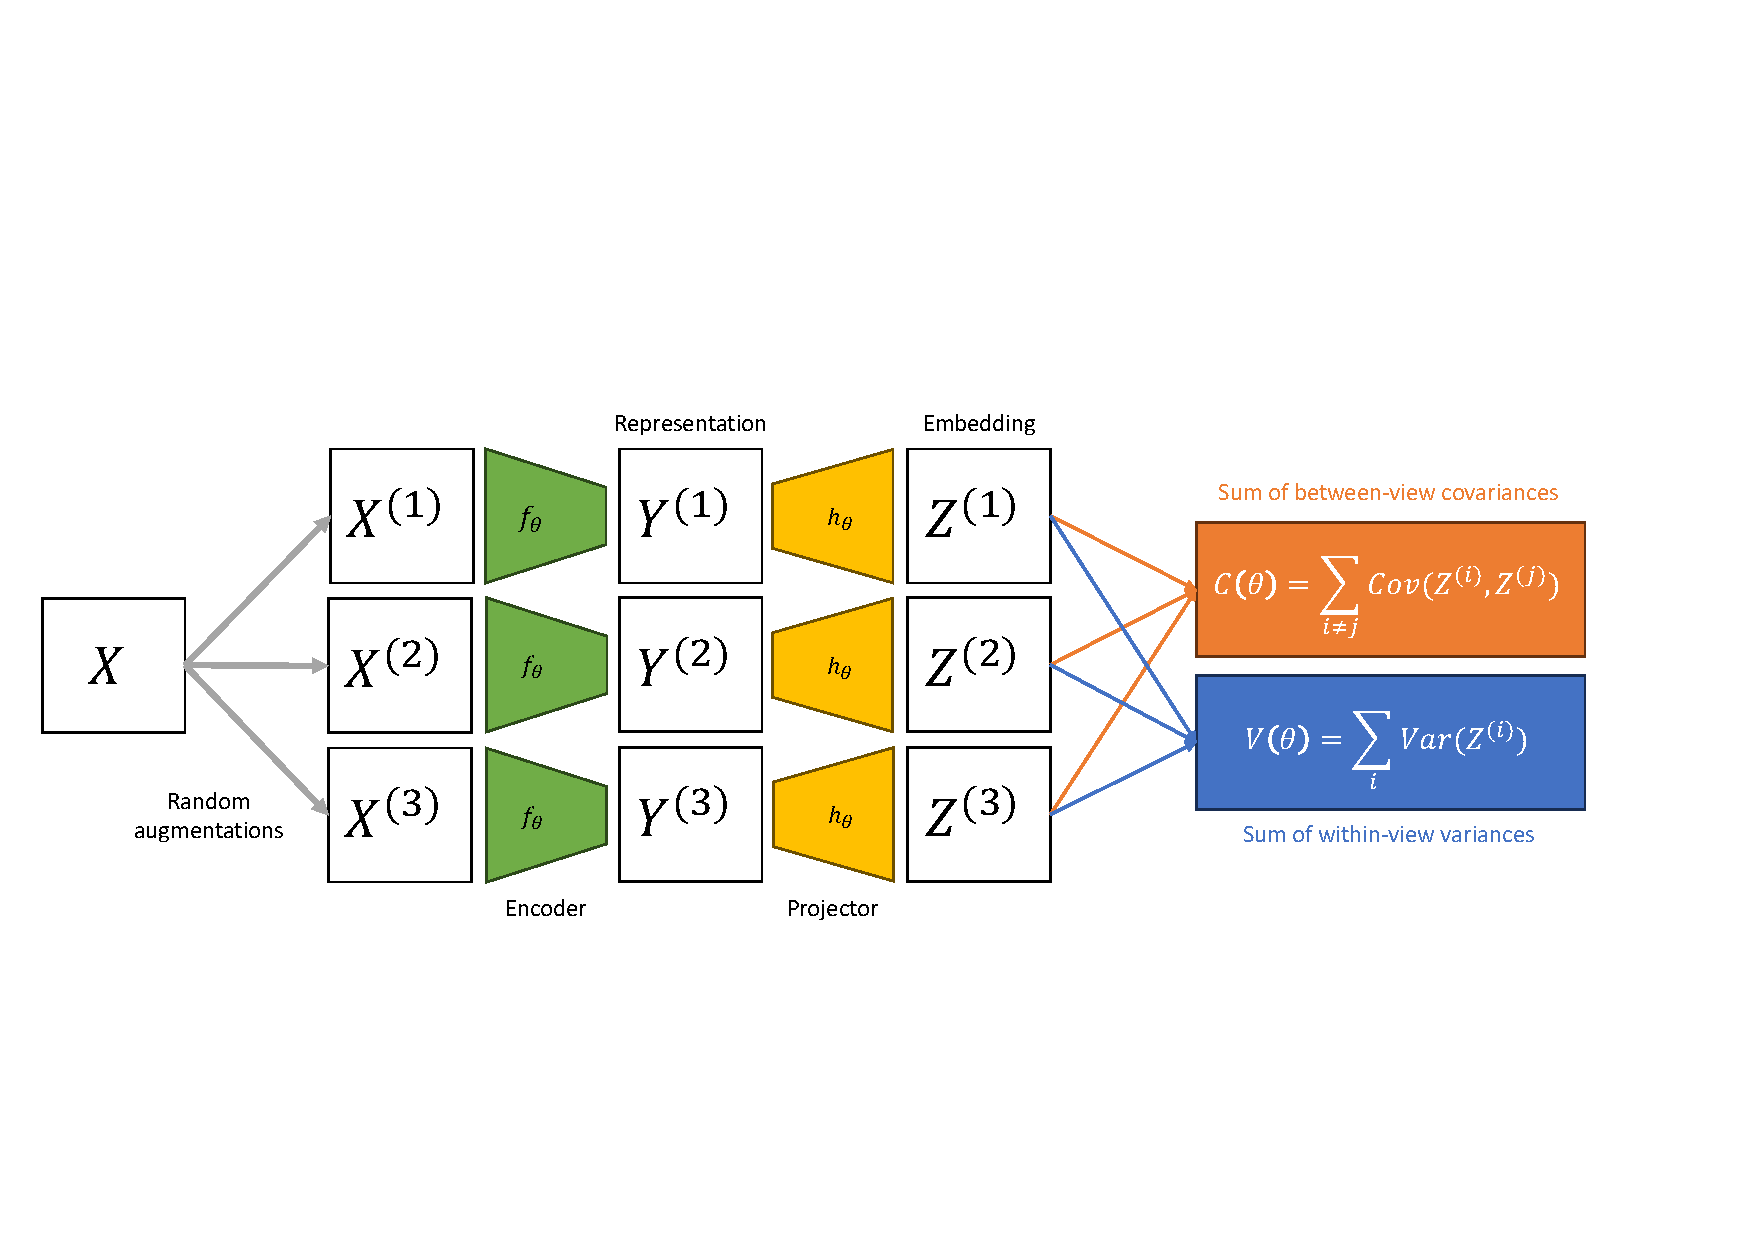
\includegraphics[width=0.9\textwidth]{figures/ssl_schematic}
\caption{Encoder-Projector Model in SSL}
\label{fig:sslschematic}
\end{figure}

\subsubsection{CCA-based SSL Methods: Barlow Twins and VICReg}
Two prominent SSL methods, Barlow Twins and VICReg, use objectives similar to CCA principles:

\textbf{Barlow Twins Loss:}
\begin{equation}
\LBT = \underbrace{\gamma \mathbb{E} \norm{Z^{(1)} - Z^{(2)}}^2}_{\text{Invariance}} + \underbrace{\beta \sum_{\substack{k,l=1 \\ k \neq l}}^K \Cov(\hat{Z}^{(i)}_k, \hat{Z}^{(i)}_l)^2}_{\text{Redundancy Reduction}}
\end{equation}

\textbf{VICReg Loss:}
\begin{equation}
\begin{split}
\LVR = &\underbrace{\gamma \mathbb{E} \norm{Z^{(1)} - Z^{(2)}}^2}_{\text{Invariance}} + \\
&\underbrace{\sum_{i \in \{1,2\}} \alpha \sum_{k=1}^K \left(1 - \sqrt{\Var(Z^{(i)}_k)}\right)_+}_{\text{Variance}} + 
\underbrace{\beta \sum_{\substack{k,l=1 \\ k \neq l}}^K \Cov(Z^{(i)}_k, Z^{(i)}_l)^2}_{\text{Covariance}}
\end{split}
\end{equation}

These methods aim to learn representations that are invariant to data augmentations while maintaining informative and decorrelated features.

\section{Methods: DCCA-EY and SSL-EY, extending GEP-EY to Deep Learning}

Building upon the Eckart-Young inspired objective introduced in the previous chapter, we now extend our approach to non-linear transformations of the data. The key idea is to replace linear representations with non-linear ones, effectively optimizing the representation of the original data to maximize canonical correlations.

Recall the objective function from the previous chapter:
\begin{align}
\LEY(\theta) = -2 \Tr C(\theta) + \norm{V_\alpha(\theta)}_F^2
\end{align}
In this chapter, we consider non-linear transformations of the data, defined as:
\begin{align}
Z^{(i)} = f^{(i)}(X^{(i)}; \theta^{(i)})
\end{align}
where $f^{(i)}$ are non-linear functions (typically neural networks) parameterized by $\theta^{(i)}$.

\subsection{Deep Multiview Canonical Correlation Analysis (DCCA-EY)}

We first show that our objective recovers Deep Multi-view CCA at any local optimum, assuming a final linear layer in each neural network.

\begin{restatable}{lemma}{recoverDeepCCA}[Objective recovers Deep Multi-view CCA]\label{lem:recover-DeepCCA}
    Assume that there is a final linear layer in each neural network $f\sps{i}$.
    Then at any local optimum, $\hat{\theta}$, of the population problem, we have
    \begin{align*}
        \LEY(\hat{\theta}) = - \norm{\MCCA_K(\hat{Z})}_2^2
    \end{align*}
    where $\hat{Z} = f_{\hat{\theta}}(X)$.
    Therefore, $\hat{\theta}$ is also a local optimum of objectives from \citet{andrew2013deep, somandepalli2019multimodal} as defined in \cref{eq:DMCCA-def}.
\end{restatable}

\begin{proof}[Proof sketch:]
    Consider treating the penultimate-layer representations as fixed, and optimising over the weights in the final layer.
    This is precisely equivalent to optimising the Eckhart-Young loss for linear CCA where the input variables are the penultimate-layer representations.
    So by \cref{prop:no-spurious}, a local optimum is also a global optimum, and by \cref{prop:EY-charac} the optimal value is the negative sum of squared generalised eigenvalues.
\end{proof}

This result shows that our objective, which we call \textbf{DCCA-EY}, is a valid generalization of Deep CCA and can be used to learn correlated non-linear representations.

\subsection{Application to Self-Supervised Learning (SSL-EY)}

We can directly apply the DCCA-EY approach to the self-supervised learning (SSL) setting, which we call \textbf{SSL-EY}. The key differences between DCCA-EY and SSL-EY are:

\begin{enumerate}
    \item Data source: In SSL-EY, the two views are augmented versions of a single sample, whereas in DCCA-EY, they are separate views of the data.
    \item Encoder architecture: SSL-EY uses the same encoder for both views as a regularization strategy, while DCCA-EY uses separate encoders for each view.
\end{enumerate}

The use of a shared encoder in SSL-EY is motivated by the fact that the paired data are generated from applying independent, identically distributed (i.i.d.) augmentations to the same original input. This approach acts as a regularizer and is intuitively sensible given that the distributions of both views are identical.

Our loss function for both DCCA-EY and SSL-EY bears some resemblance to those of Barlow Twins and VICReg:

\begin{align*}
    \LEY(\theta) = - 2 \tr C(\theta) + \norm{V_\alpha(\theta)}_F^2
\end{align*}

where $C(\theta)$ is the cross-covariance matrix between the representations of the views, and $V_\alpha(\theta)$ is a matrix involving the individual covariance matrices of each view.

This objective has two terms:
\begin{enumerate}
    \item $- 2 \tr C(\theta)$: encourages correlated representations across views, similar to the invariance term in Barlow Twins and VICReg.
    \item $\norm{V_\alpha(\theta)}_F^2$: involves individual covariance matrices, analogous to the variance and covariance terms in VICReg.
\end{enumerate}

The main difference is that our method is based on canonical correlation principles, which may offer additional benefits in terms of representation quality and interpretability.

\subsection{PyTorch Implementation}

We provide a unified PyTorch implementation for both DCCA-EY and SSL-EY in Listing \ref{lst:pytorch-unified}. This implementation defines a single class that can be used for both methods, with the key difference being in how the encoders are initialized and used.

\begin{listing}[ht]
    \begin{minted}{python}
import torch
import torch.nn as nn

class UnifiedEY(nn.Module):
    def __init__(self, encoders, ssl_mode=False):
        super(UnifiedEY, self).__init__()
        self.ssl_mode = ssl_mode
        if ssl_mode:
            assert len(encoders) == 1, "SSL mode requires a single encoder"
            self.encoder = encoders[0]
        else:
            self.encoders = nn.ModuleList(encoders)

    def forward(self, Xs):
        if self.ssl_mode:
            Zs = [self.encoder(X) for X in Xs]
        else:
            Zs = [encoder(X) for encoder, X in zip(self.encoders, Xs)]
        return Zs

    def loss(self, Zs, alphas=[0, 0]):
        # Compute total between-view covariance matrix
        C = torch.zeros(Zs[0].shape[1], Zs[0].shape[1])
        for i in range(len(Zs)):
            for j in range(i + 1, len(Zs)):
                C += torch.matmul(Zs[i].T, Zs[j]) / Zs[i].shape[0]
        
        # Compute total within-view variance matrix
        V = torch.zeros(Zs[0].shape[1], Zs[0].shape[1])
        for i, alpha in enumerate(alphas):
            Vi = torch.matmul(Zs[i].T, Zs[i]) / Zs[i].shape[0]
            V += alpha * torch.eye(Vi.shape[0]) + (1 - alpha) * Vi
        
        # Compute loss
        loss = -2 * torch.trace(C) + torch.norm(V, p='fro') ** 2
        
        return loss
    \end{minted}
    \caption{Unified PyTorch implementation for DCCA-EY and SSL-EY.}
    \label{lst:pytorch-unified}
\end{listing}

This unified implementation can be used for both DCCA-EY and SSL-EY by setting the \texttt{ssl\_mode} parameter appropriately. When \texttt{ssl\_mode=True}, it uses a single shared encoder for both views (SSL-EY), and when \texttt{ssl\_mode=False}, it uses separate encoders for each view (DCCA-EY).

In the next section, we will present experiments demonstrating the effectiveness of our DCCA-EY and SSL-EY methods in their respective settings.

\section{Experiments and Results}

\subsection{Deep CCA}\label{sec:experiments-DCCA}
In this experiment, we aim to establish the superiority of our DCCA-EY method over existing Deep Canonical Correlation Analysis approaches.
We specifically focus on showcasing how DCCA-EY outperforms these methods in terms of correlation capture, convergence speed, and ease of hyperparameter tuning.
The experimental setup is aligned with that of \citet{wang2015stochastic}, providing a direct comparison under identical conditions.

As per \citet{wang2015stochastic}, our architecture comprises multilayer perceptrons with two hidden layers of size 800 and an output layer of 50 with ReLU activations.
We train these networks for 20 epochs.
However, our primary goal is to learn $K=50$ dimensional representations over a range of mini-batch sizes (from 20 to 100) across 50 epochs, demonstrating the robustness and scalability of DCCA-EY even in varying batch conditions.

In this chapter, we employ the Total Correlation Captured (TCC) metric for evaluation.
While similar to the PCC metric described in the previous chapter, TCC does not rely on a ground truth for its computation.
Instead, it is defined as \( \text{TCC} = \sum_{k=1}^K \rho_k \), where $\rho_k$ are the empirical correlations between the neural network-based representations $Z^{(i)} = f^{(i)}(X^{(i)})$ on a validation set, rather than on the training set as was the case with PCC. This distinction is crucial as TCC evaluates the model's performance in capturing correlations in an unseen dataset, offering a more robust measure of its generalization capability.
\subsubsection{Data}
The Split MNIST dataset is a modified version of the original MNIST dataset, where each 28x28 pixel grayscale image of handwritten digits (0-9) is divided into left and right halves, creating two distinct views.
This split challenges models to learn from partial information, as each view contains only half of the digit, either the left or the right side.
The dataset comprises 50,000 training and 10,000 test images.
The X-Ray Microbeam Speech Production Database (XRMB) is a multi-view dataset used for studying articulatory speech data.
It comprises around 40,000 spoken utterances from 47 American English speakers.
The dataset provides two views: acoustic features and articulatory measurements.
The acoustic features consist of 273-dimensional vectors representing spectral characteristics, while the articulatory measurements include 112-dimensional vectors capturing the position and movement of speech articulators (like the tongue and lips).
The XRMB dataset is notable for its complexity and high dimensionality, making it a challenging testbed for multiview learning algorithms.

\subsubsection{Parameters} For each method, we searched over a hyperparameter grid using \citet{wandb}.

\begin{table}[h!]
    \centering
    \begin{tabular}{|l|l|}
        \hline Parameter           & Values           \\
        \hline minibatch size      & 100, 50, 20      \\
        \hline lr                  & 1e-3, 1e-4, 1e-5 \\
        \hline $\rho$\footnotemark & 0.6, 0.8, 0.9    \\
        \hline epochs              & 50               \\
        \hline
    \end{tabular}
    \footnotetext{$\rho$ is only used for DCCA-NOI}\label{tab:hyperparams}
\end{table}

\subsubsection{Observations on SplitMNIST}
For the SplitMNIST dataset, Figure~\ref{fig:corr_mnist} shows the comparison of methods across different batch sizes.
We observe that DCCA-STOL captures significantly less correlation than the other methods and breaks down when the mini-batch size is smaller than the dimension $K=50$.
Figure~\ref{fig:lr_mnist} illustrates the learning progress over 50 epochs, where DCCA-NOI, despite performing similarly to DCCA-EY, requires more careful hyperparameter tuning and demonstrates a slower convergence speed.

\subsubsection{Observations on XRMB}
On the XRMB dataset, as seen in Figure~\ref{fig:corr_xrmb}, similar trends are evident.
DCCA-STOL struggles with smaller mini-batch sizes, while DCCA-NOI, though comparable to DCCA-EY in performance, lags in convergence speed, as shown in Figure~\ref{fig:lr_xrmb}.

\begin{figure}
    \centering
    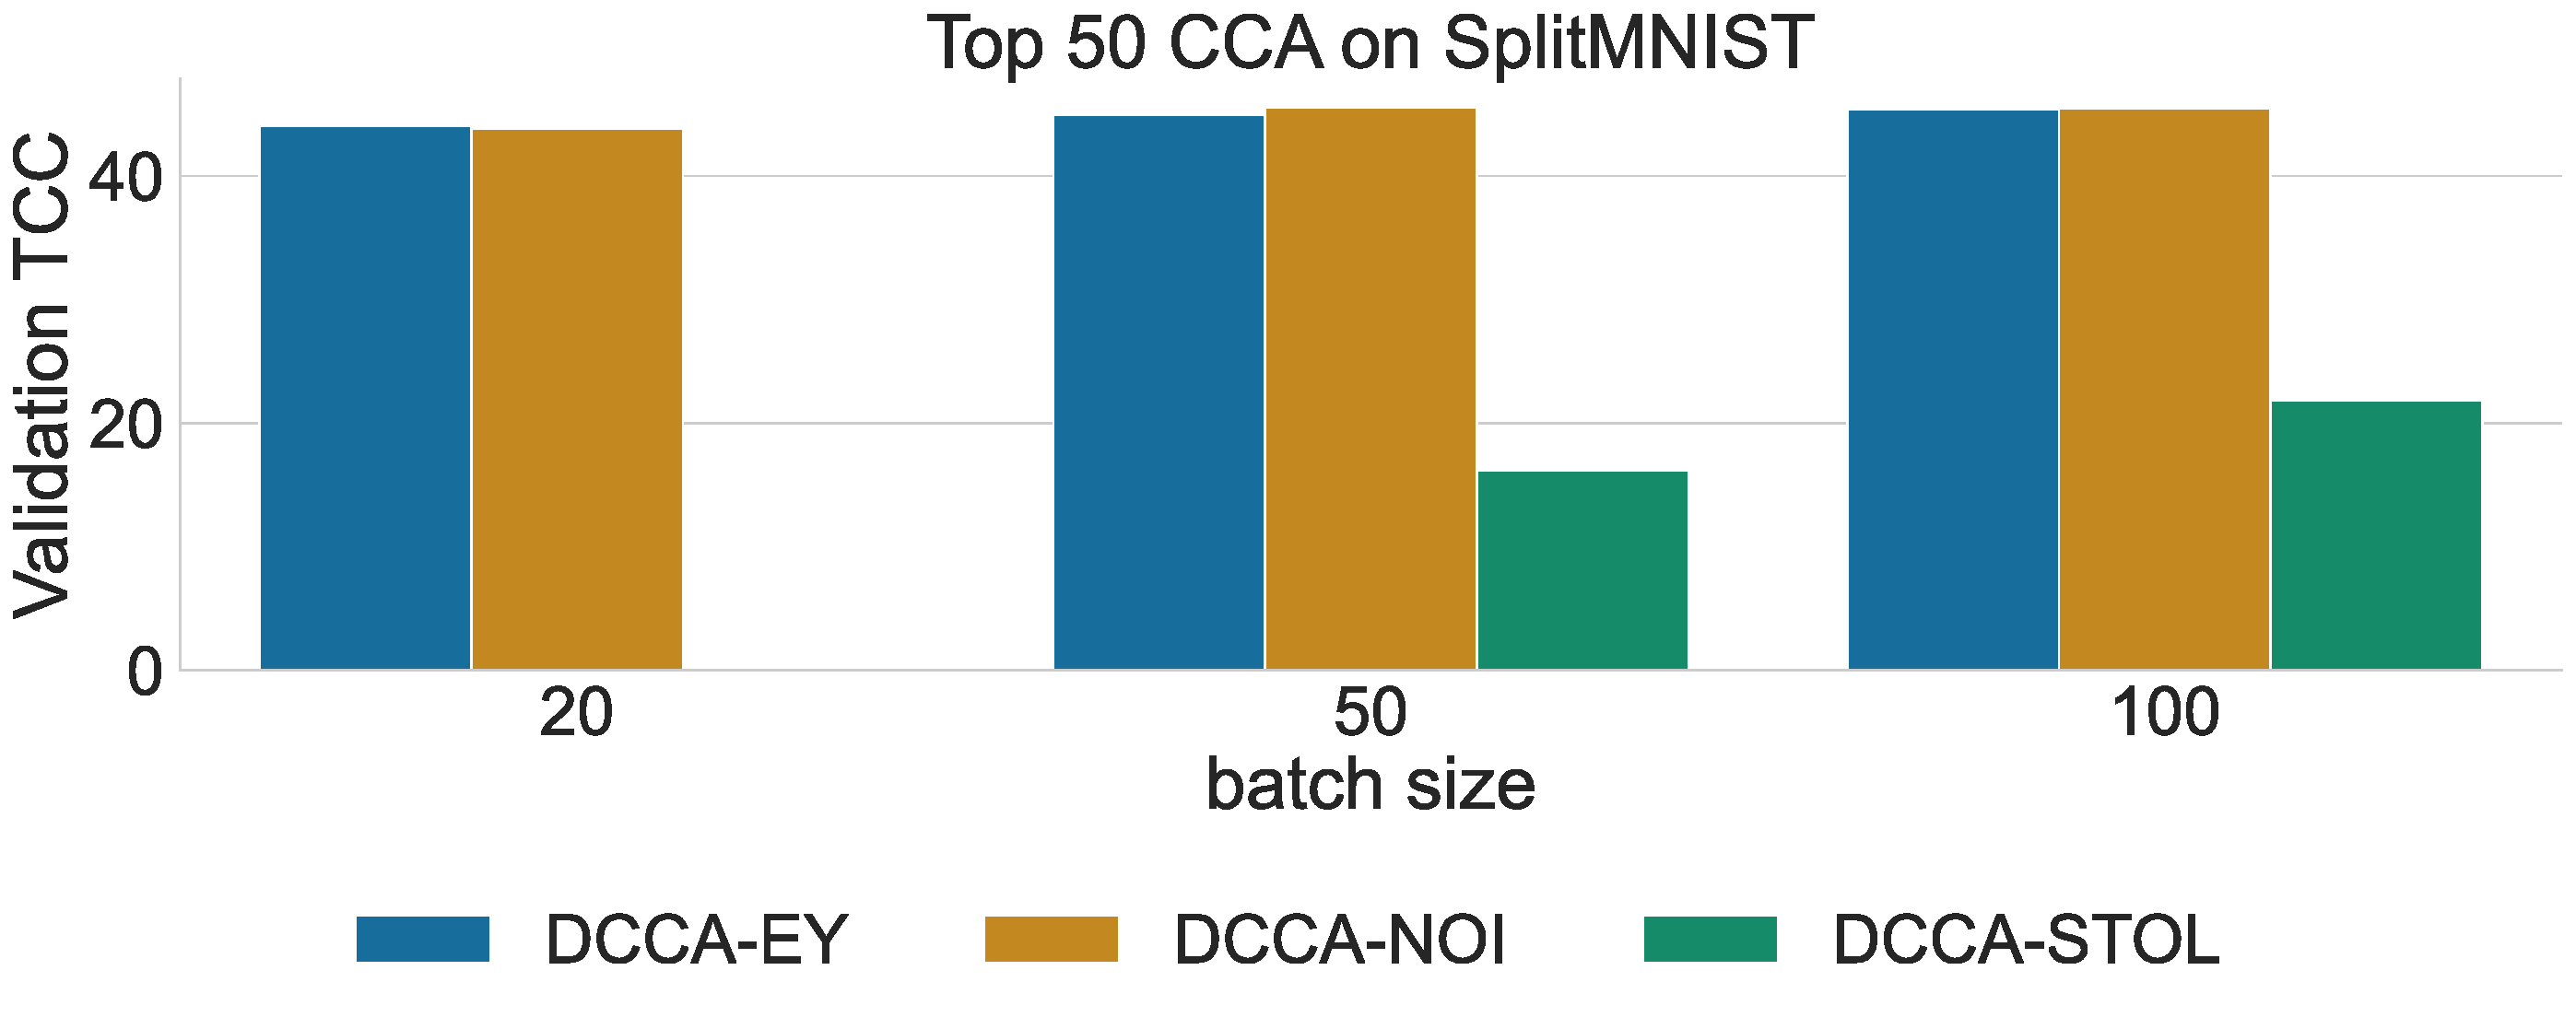
\includegraphics[width=0.8\textwidth]{figures/DCCA/SplitMNIST_models_different_batch_sizes}
    \caption{Deep CCA on SplitMNIST: Comparison of methods across varying batch sizes.}
    \label{fig:corr_mnist}
\end{figure}

\begin{figure}
    \centering
    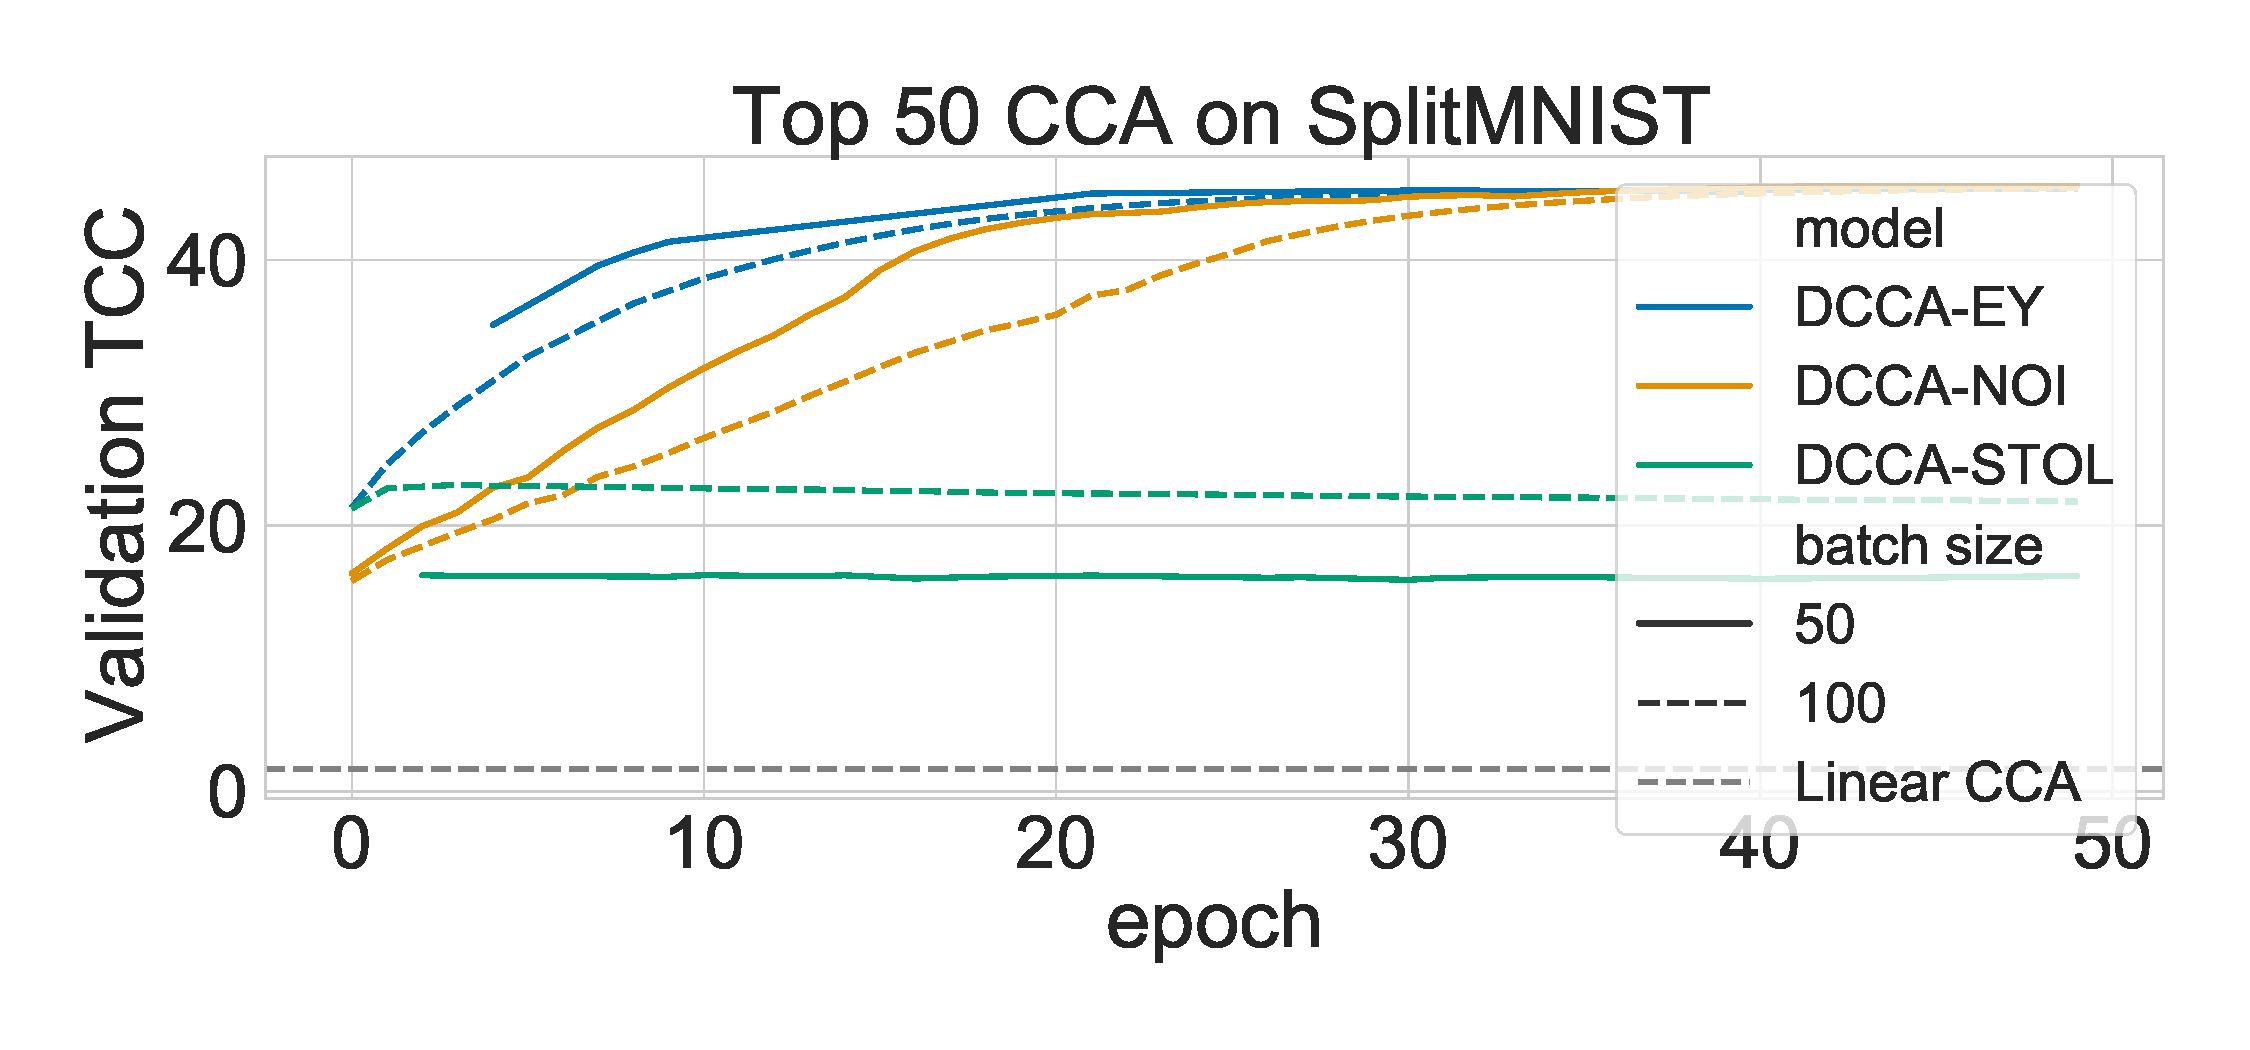
\includegraphics[width=0.8\textwidth]{figures/DCCA/SplitMNIST_allbatchsizes_pcc}
    \caption{Deep CCA on SplitMNIST: Learning progress over 50 epochs.}
    \label{fig:lr_mnist}
\end{figure}

\begin{figure}
    \centering
    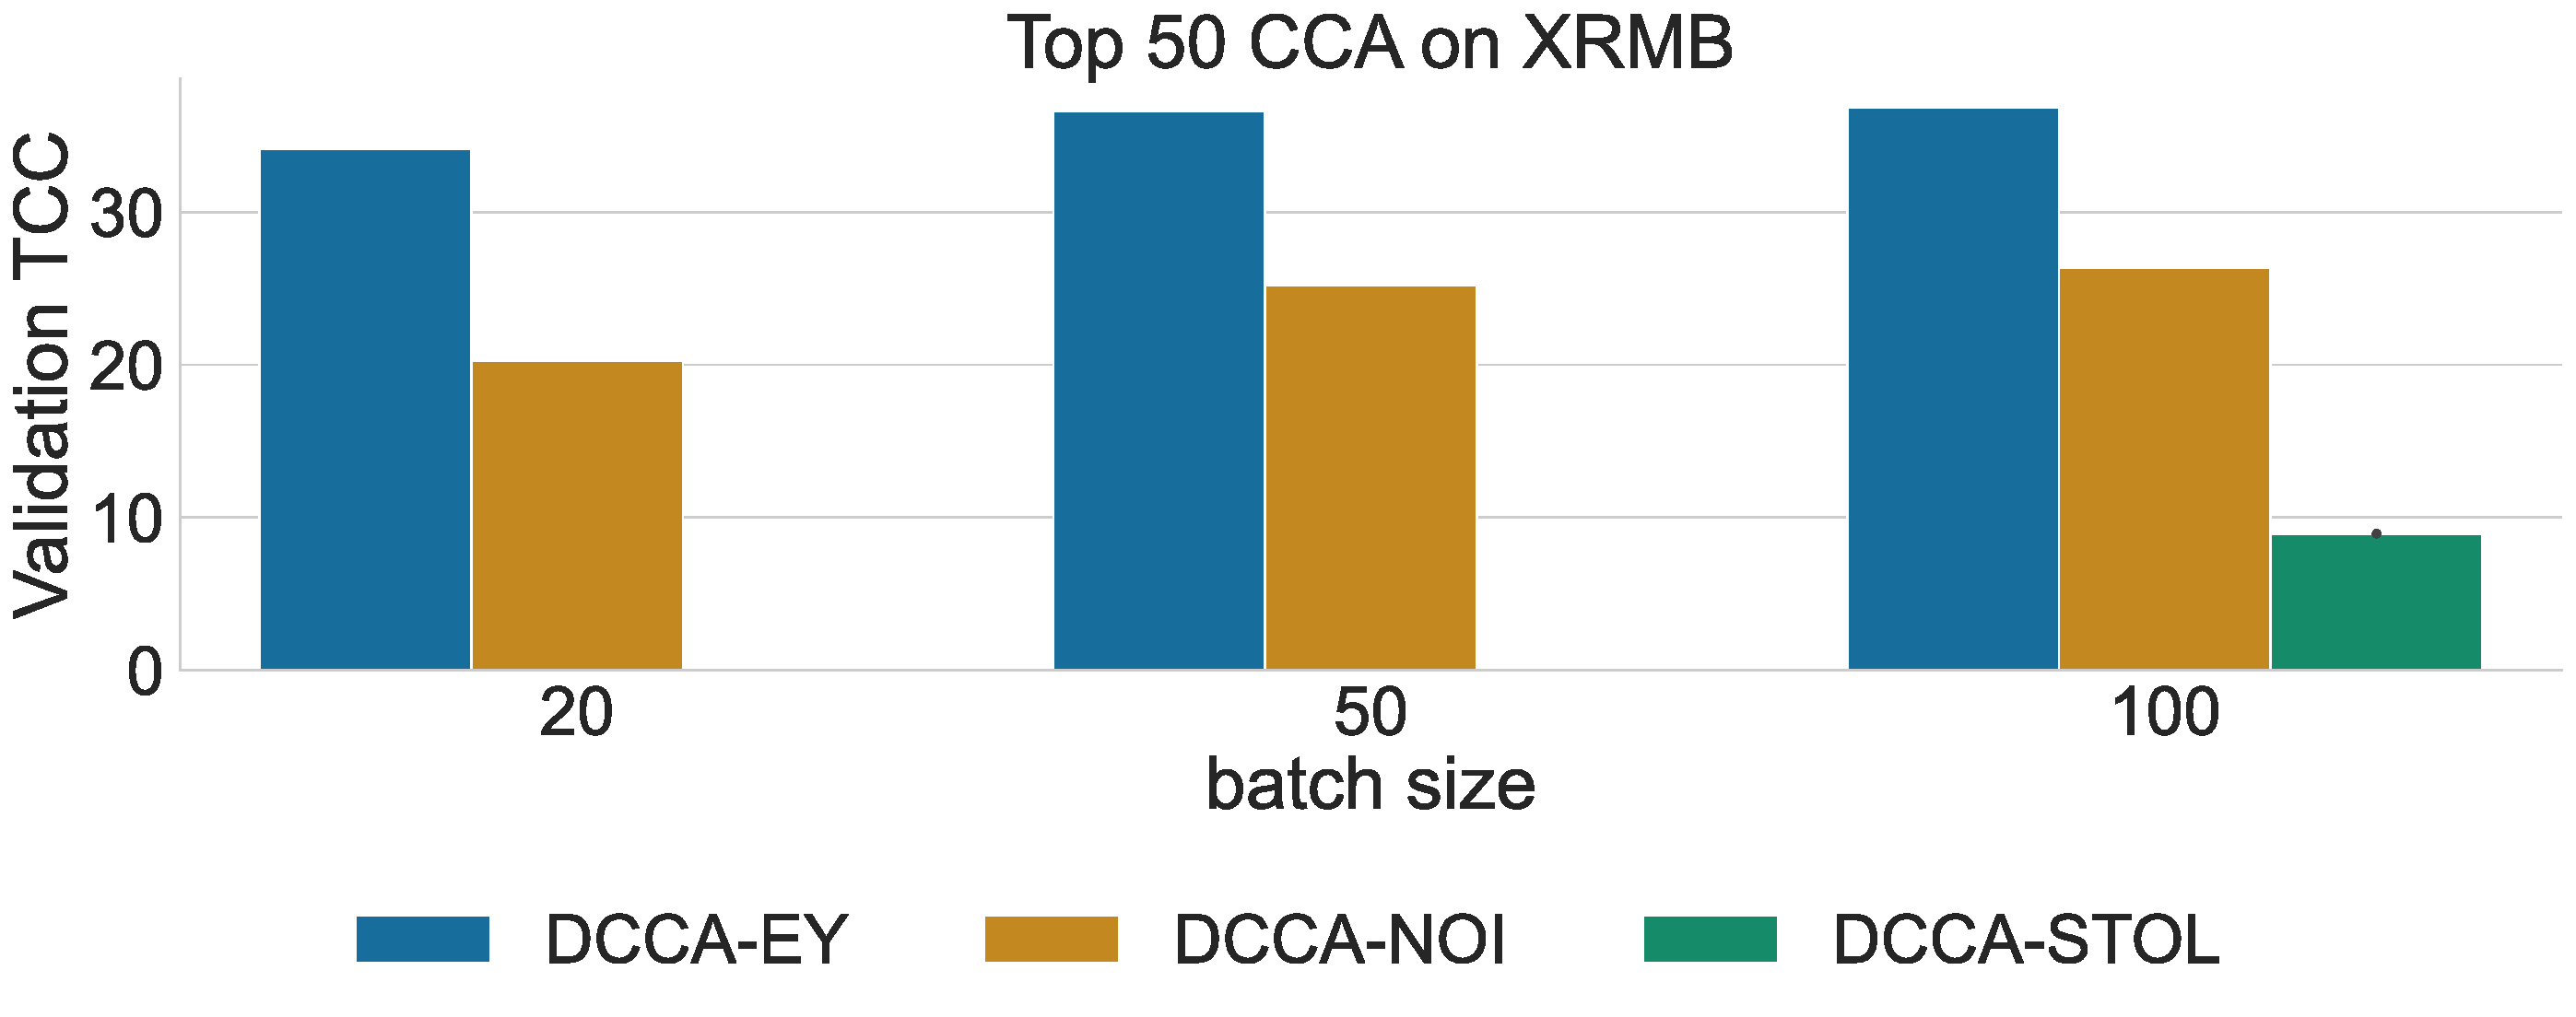
\includegraphics[width=0.8\textwidth]{figures/DCCA/XRMB_models_different_batch_sizes}
    \caption{Deep CCA on XRMB: Comparison of methods across varying batch sizes.}
    \label{fig:corr_xrmb}
\end{figure}

\begin{figure}
    \centering
    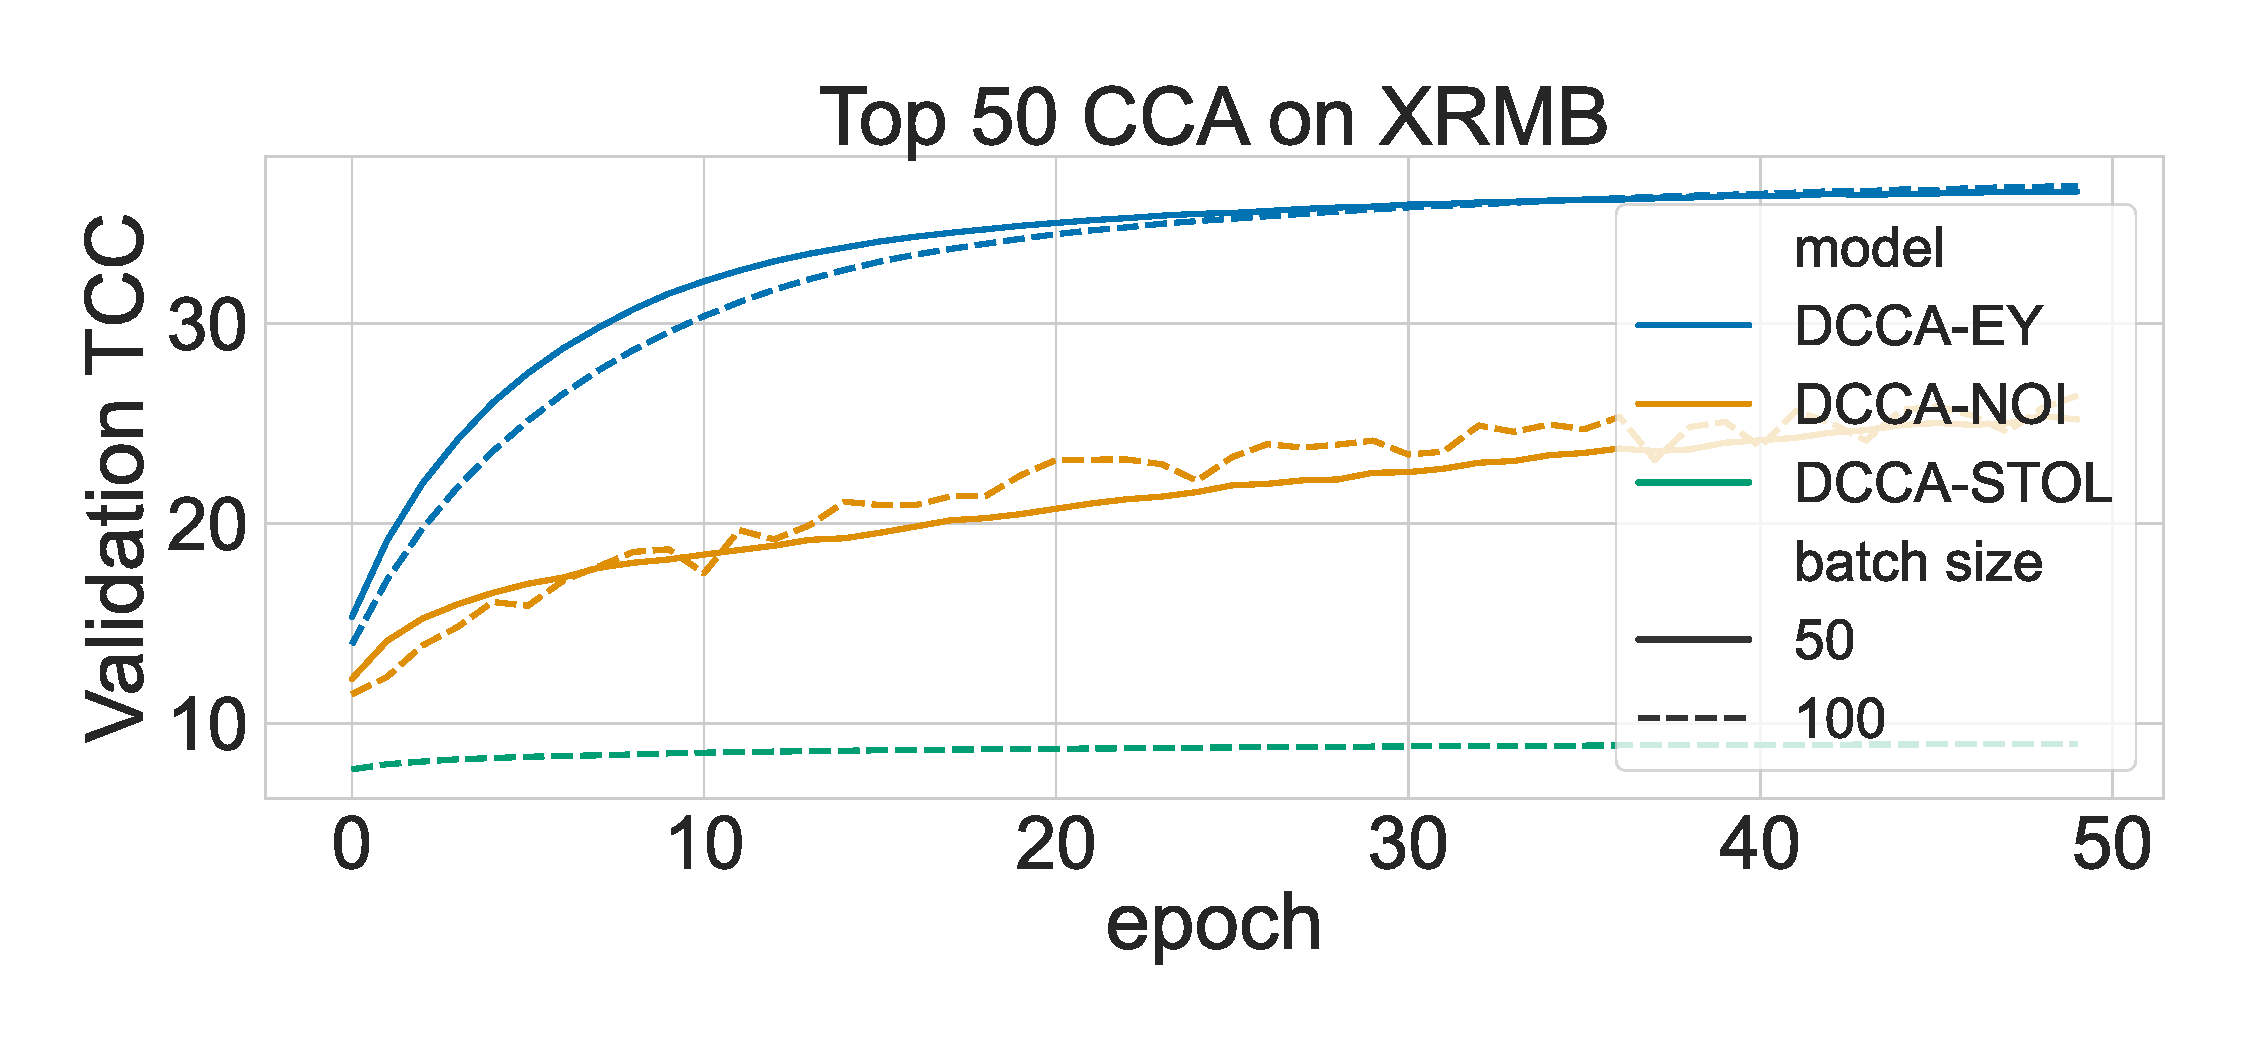
\includegraphics[width=0.8\textwidth]{figures/DCCA/XRMB_allbatchsizes_pcc}
    \caption{Deep CCA on XRMB: Learning progress over 50 epochs.}
    \label{fig:lr_xrmb}
\end{figure}

\subsection{Deep Multiview CCA: Robustness Across Different Batch Sizes}
In our second experiment, our objective is to showcase the adaptability and effectiveness of the DCCA-EY method in the multiview context, particularly in comparison to existing methods such as Deep MCCA and Deep GCCA.
We again learn $K=50$ dimensional representations, but now train for 100 epochs.
We employ a multiview extension of the Total Correlation Captured (TCC) metric, termed Total Multiview Correlation Captured (TMCC). TMCC averages the correlation across views and is defined using the consistent notation from \cref{sec:background-unified} as:
\[
    \text{TMCC} = \sum_{k=1}^{K} \frac{1}{I(I-1)} \sum_{\substack{i,j \leq I \\ i \neq j}} \text{corr}(Z_k^{(i)}, Z_k^{(j)}),
\]
where \( Z_k^{(i)} \) represents the \( k \)-th dimension of the \( i \)-th view's representation.
This metric effectively measures the extent to which our method captures correlations between different views in a multidimensional representation space.

\subsubsection{Data} We choose the mfeat dataset \citep{misc_multiple_features_72} for this purpose, which comprises 2,000 handwritten numeral patterns represented through six distinct feature sets, including Fourier coefficients, profile correlations, Karhunen-Love coefficients, pixel averages in \(2 \times 3\) windows, Zernike moments, and morphological features.
These diverse features present an ideal testbed for evaluating the performance of multiview learning methods.

\subsubsection{Parameters} For each method, we searched over a hyperparameter grid using \citet{wandb}.

\begin{table}[h!]
    \centering
    \begin{tabular}{|l|l|}
        \hline Parameter      & Values                       \\
        \hline minibatch size & 5,10,20,50,100,200           \\
        \hline components     & 50                           \\
        \hline epochs         & 100                          \\
        \hline lr             & 0.01, 0.001, 0.0001, 0.00001 \\
        \hline
    \end{tabular}
\end{table}

\subsubsection{Observations}
Figure~\ref{fig:dmcca_corr} illustrates the comparison of DCCA-EY with Deep GCCA and Deep MCCA across different mini-batch sizes, using the validation TMCC metric.
DCCA-EY consistently outperforms both Deep GCCA and Deep MCCA, showcasing its superior ability to capture validation TMCC. Notably, Deep MCCA encounters issues when the batch size is smaller than $K=50$, likely due to singular empirical covariances.
Deep GCCA, while not breaking down, significantly underperforms with smaller batch sizes, highlighting limitations in scalability and efficiency for large-scale data applications.

In Figure~\ref{fig:dmcca_lr}, we observe the learning curves for batch sizes 50 and 100. Both Deep MCCA and Deep GCCA demonstrate rapid initial learning of significant correlations but reach a plateau relatively quickly. In contrast, DCCA-EY exhibits a consistent improvement over time and notably outperforms the other methods by the end of the training period. This behavior underscores the enhanced learning capability and efficiency of DCCA-EY, especially in the context of large-scale, high-dimensional data.

\begin{figure}
    \centering
    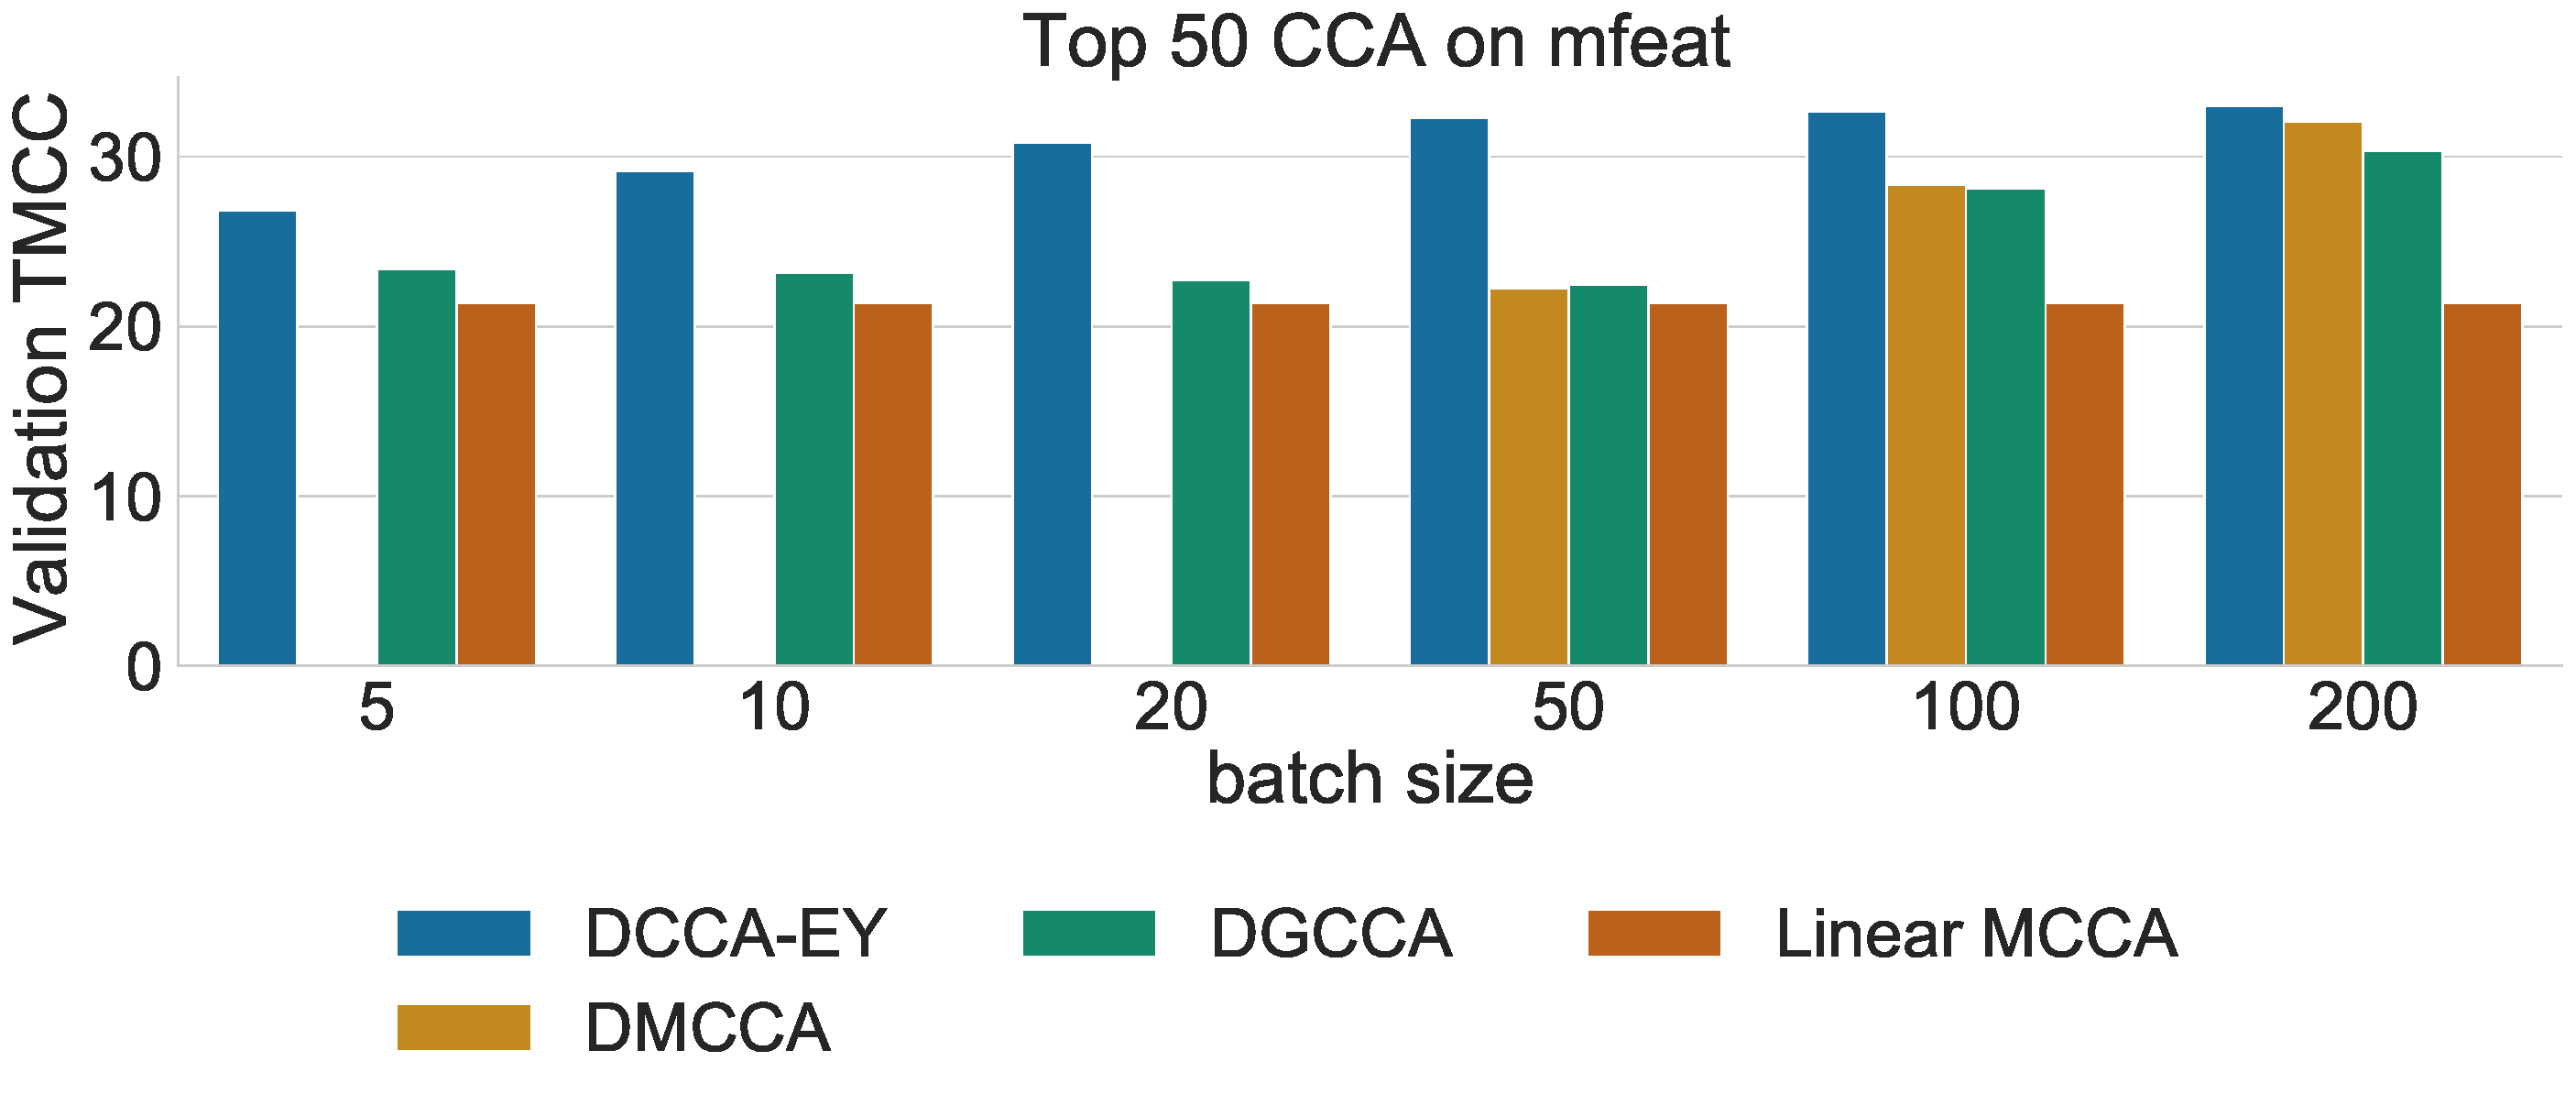
\includegraphics[width=0.8\textwidth]{figures/DMCCA/mfeat_models_different_batch_sizes}
    \caption{Deep Multi-view CCA on mfeat: Comparison across various mini-batch sizes using the Validation TMCC metric.}\label{fig:dmcca_corr}
\end{figure}

\begin{figure}
    \centering
    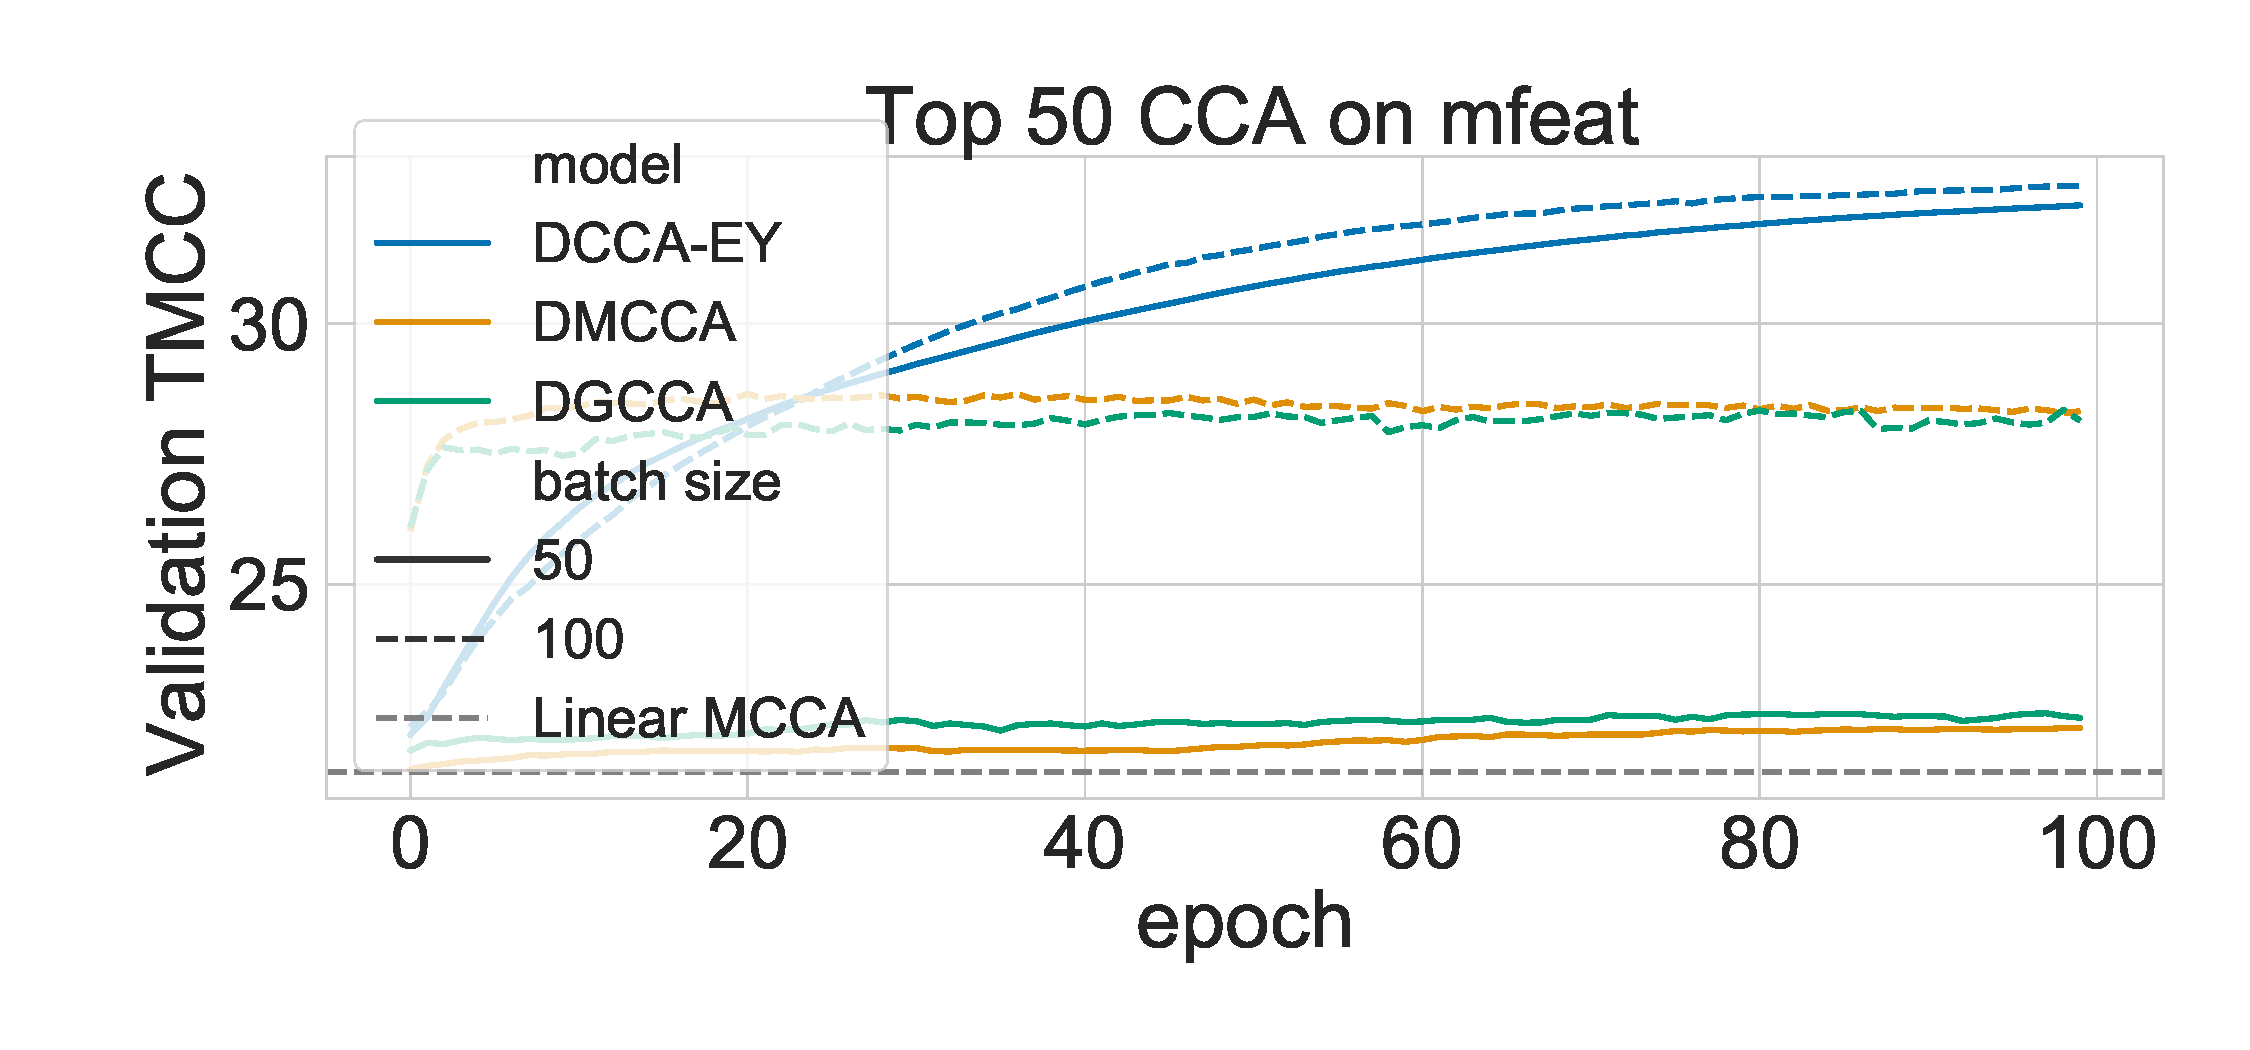
\includegraphics[width=0.8\textwidth]{figures/DMCCA/mfeat_allbatchsizes_pcc}
    \caption{Deep Multi-view CCA on mfeat: Learning progress over 100 epochs for batch sizes 50 and 100.}\label{fig:dmcca_lr}
\end{figure}

\subsection{Self-Supervised Learning with SSL-EY}
Finally, we benchmark our self-supervised learning algorithm, SSL-EY, with Barlow Twins and VICReg on standard SSL benchmarks.
We follow a standard experimental design \citep{tong2023emp}.
Indeed, we use the sololearn library \citep{da2022solo}, which offers optimized setups particularly tailored for VICReg and Barlow Twins.
All methods use a ResNet-18 encoder coupled with a bi-layer projector network.
Training spans 1,000 epochs with batches of 256 images.
For SSL-EY, we use the hyperparameters optimized for Barlow Twins, aiming not to outperform but to showcase the robustness of our method.
We predict labels via a linear probe on the learnt representations and evaluate performance with Top-1 and Top-5 accuracies on the validation set.

\subsubsection{Data} We use the CIFAR-10 and CIFAR-100 datasets, which comprise 60,000 labelled images of size 32x32.
CIFAR-10 contains 10 classes, while CIFAR-100 contains 100 classes.

\subsubsection{Observations} As Table \ref{tab:selfsup} demonstrates, SSL-EY rivals Barlow Twins and VICReg, despite employing general hyperparameters as opposed to the latter's specifically optimized ones.

\begin{table}[H]
    \centering
    \caption{Comparing the performance of SSL methods on CIFAR-10 and CIFAR-100.}
    \resizebox{\textwidth}{!}{%
    \begin{tabular}{|l|c|c|c|c|}
        \hline
        Method          & CIFAR-10 Top-1 & CIFAR-10 Top-5 & CIFAR-100 Top-1 & CIFAR-100 Top-5 \\
        \hline
        Barlow Twins    & \textbf{92.1}  & 99.73          & \textbf{71.38}  & \textbf{92.32}  \\
        \hline
        VICReg          & 91.68          & 99.66          & 68.56           & 90.76           \\
        \hline
        \textbf{SSL-EY} & 91.43          & \textbf{99.75} & 67.52           & 90.17           \\
        \hline
    \end{tabular}
    }
    \label{tab:selfsup}
\end{table}

\subsubsection{Model Convergence} In deep learning, a learning curve usually represents a graph showing the model's learning progress against number of epochs.
Figure \ref{fig:ssl_learning_curve_cifar100_top5} illustrates that the performance variations at 1,000 epochs, shown in Table \ref{tab:selfsup}, primarily stem from optimization noise, with convergence speeds being comparable among methods.

\begin{figure}[H]
    \centering
    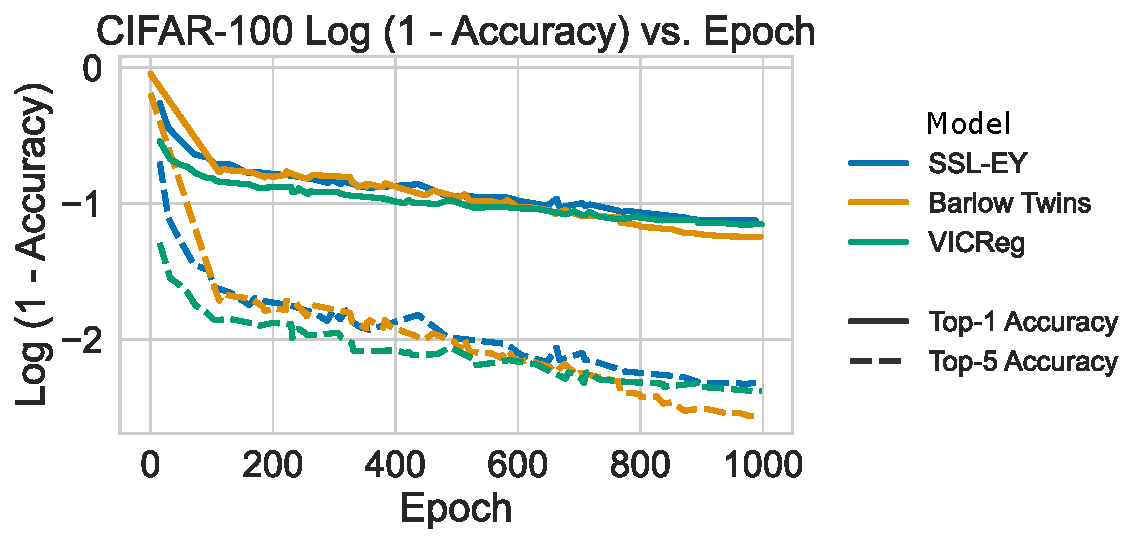
\includegraphics[width=0.8\textwidth]{figures/SSL/cifar100_learning_curve_log_error}
    \caption{Learning curves for SSL-EY, Barlow Twins, and VICReg on CIFAR-100, depicting 1,000-epoch performance.}
    \label{fig:ssl_learning_curve_cifar100_top5}
\end{figure}

\subsubsection{Projector Size Variation} We hypothesized that SSL-EY's robustness to projector size might allow for efficient performance even with smaller projectors or without one.
This hypothesis led us to experiment with varying projector output dimensions and completely removing the projector while maintaining the encoder size.
Figure \ref{fig:ssl_projector_dimensions_100} shows SSL-EY's sustained performance with reduced projector size, indicating more efficient representations compared to Barlow Twins and VICReg.
Furthermore, as Table \ref{tab:selfsup} and Figure \ref{fig:ssl_learning_curve_cifar100_vs_corr} suggest, SSL-EY performs consistently well even without a projector, underlining its reduced reliance on this architectural component.

\begin{figure}[H]
    \begin{subfigure}[b]{0.47\textwidth}
        \centering
        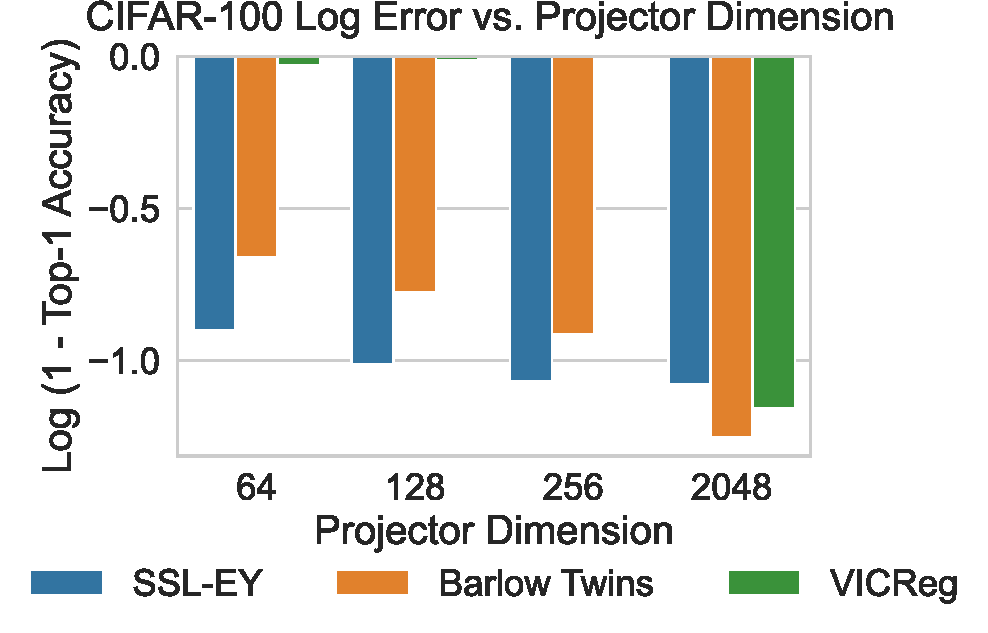
\includegraphics[width=\textwidth]{figures/SSL/cifar100_proj_dim_log_error}
        \caption{Performance of SSL-EY with varying projector dimensions on CIFAR-100.}
        \label{fig:ssl_projector_dimensions_100}
    \end{subfigure}
    \hfill
    \begin{subfigure}[b]{0.47\textwidth}
        \centering
        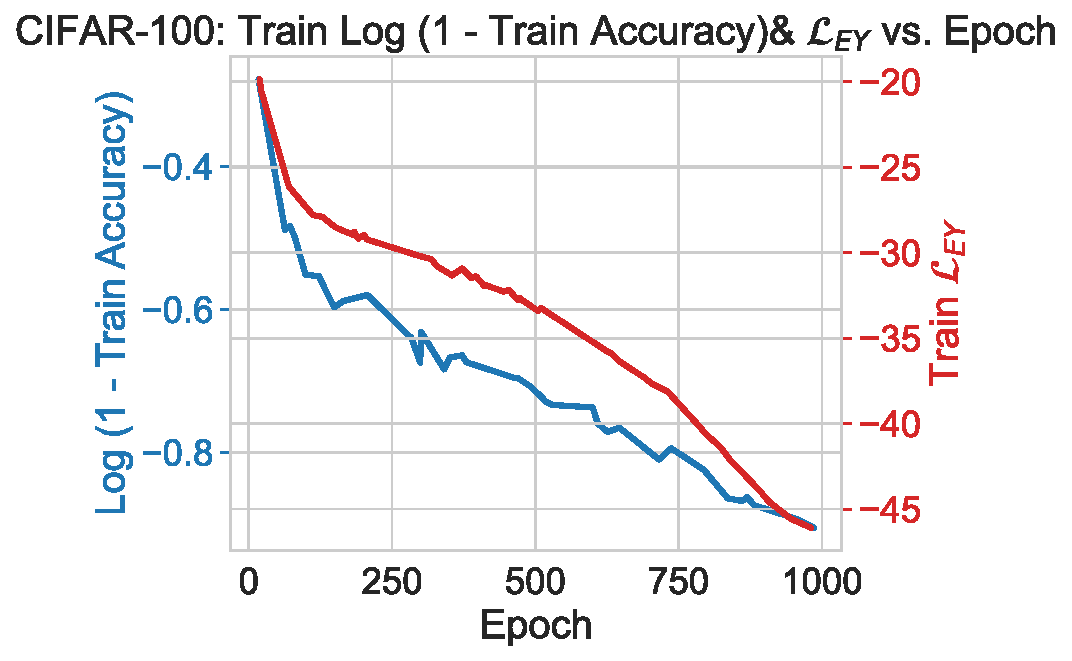
\includegraphics[width=\textwidth]{figures/SSL/cifar100_corr_vs_acc_log_error}
        \caption{Correlation of EY loss with classification accuracy in SSL-EY on CIFAR-100.}
        \label{fig:ssl_learning_curve_cifar100_vs_corr}
    \end{subfigure}
    \caption{CIFAR 100 Projector Analysis: (a) Examining the impact of projector size on SSL-EY's performance. (b) Investigating the relationship between EY loss and classification accuracy.}
    \label{fig:ssl_projector_cifar_100}
\end{figure}

\subsubsection{$\LEY$ as an Informative Metric} Figure\ref{fig:ssl_learning_curve_cifar100_vs_corr} offers two insights.
First, it evidences the close relationship between EY loss and classification accuracy, highlighting the potential of maximizing canonical correlation as a pretext task in SSL. Second, it reveals that even a reduced projector dimensionality does not reach full capacity within 1,000 epochs, implying untapped potential in SSL-EY's representation capacity.
evolution of the correlation, measured by $\LEY$, suggests a new avenue for monitoring model training, potentially eliminating the need for a separate validation task.

\begin{figure}[H]
    \centering
    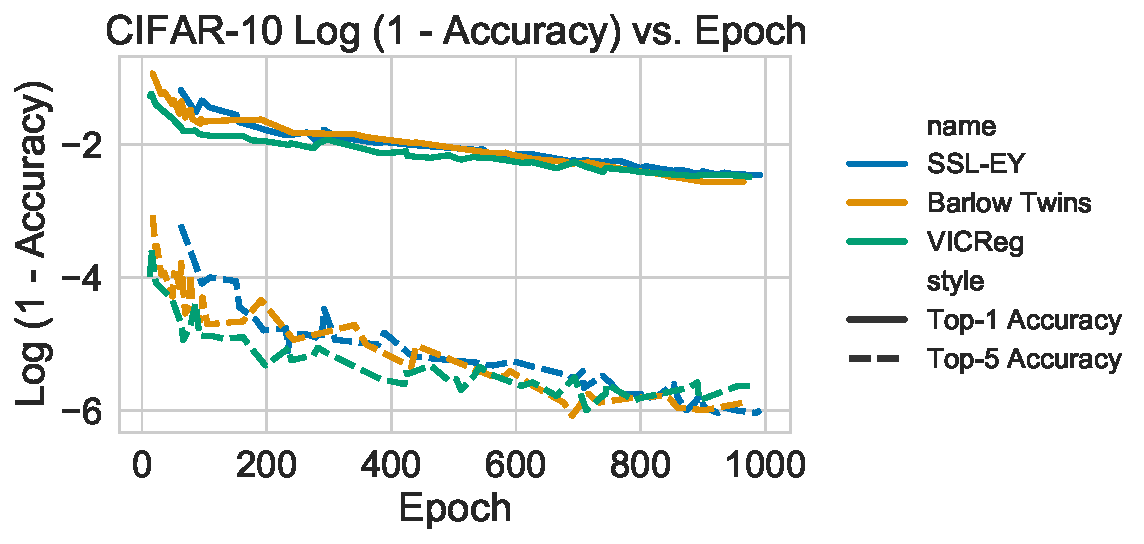
\includegraphics[width=0.57\textwidth]{figures/SSL/cifar10_learning_curve_log_error}
    \caption{Learning curves for SSL-EY, Barlow Twins, and VICReg on CIFAR-10, depicting 1,000-epoch performance.}
    \label{fig:ssl_learning_curve_cifar10_top5}
\end{figure}

\begin{figure}[H]
    \begin{subfigure}[b]{0.47\textwidth}
        \centering
        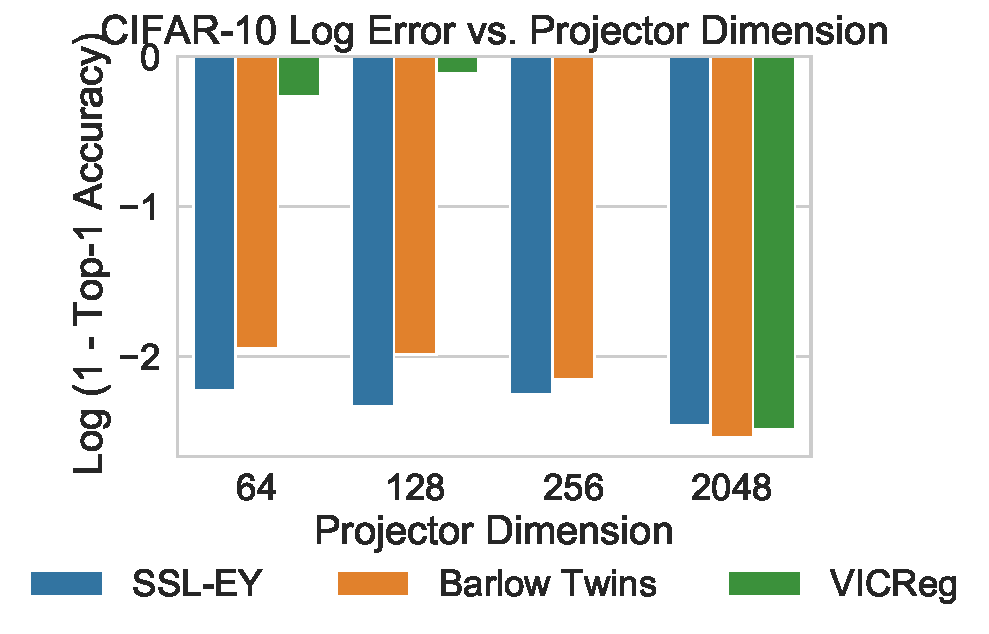
\includegraphics[width=\textwidth]{figures/SSL/cifar10_proj_dim_log_error}
        \caption{Performance of SSL-EY with varying projector dimensions on CIFAR-10.}
        \label{fig:ssl_projector_dimensions_10}
    \end{subfigure}
    \hfill
    \begin{subfigure}[b]{0.47\textwidth}
        \centering
        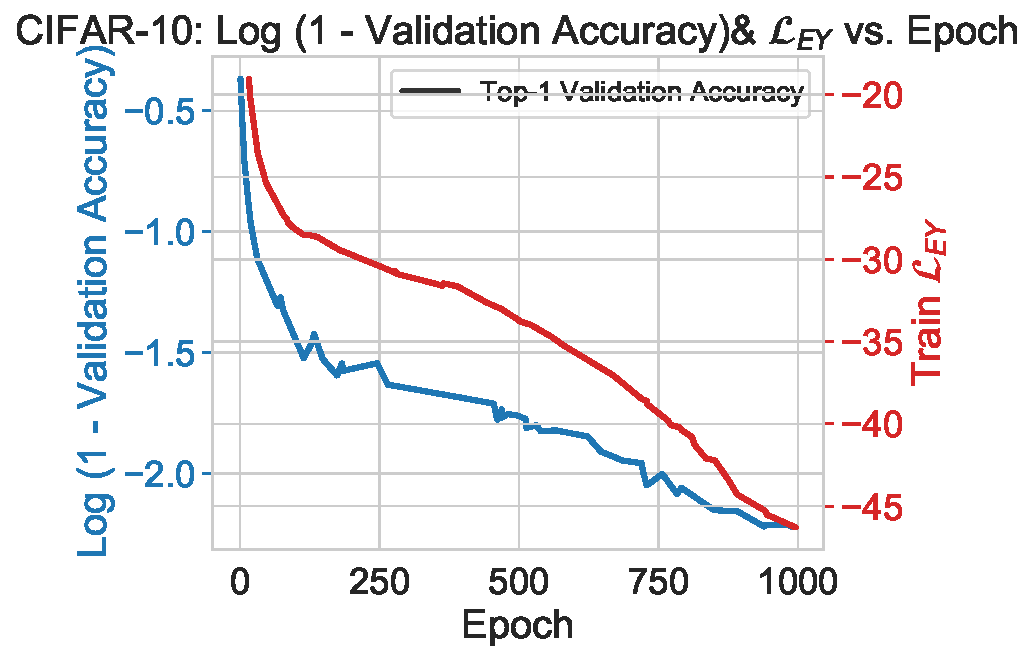
\includegraphics[width=\textwidth]{figures/SSL/cifar10_corr_vs_acc_log_error}
        \caption{Correlation of EY loss with classification accuracy in SSL-EY on CIFAR-10.}
        \label{fig:ssl_learning_curve_cifar10_vs_corr}
    \end{subfigure}
    \caption{CIFAR 10 Projector Analysis: (a) Examining the impact of projector size on SSL-EY's performance. (b) Investigating the relationship between EY loss and classification accuracy.}
    \label{fig:ssl_projector_cifar_10}
\end{figure}


\section{Discussion and Limitations}

\subsection{Limitations}

Our innovative formulation of DCCA-EY successfully addresses the limitations of traditional Deep CCA methods, particularly in stochastic settings.
The experimental results on Split MNIST and XRMB datasets demonstrate DCCA-EY's superior capability in capturing correlations efficiently across a range of mini-batch sizes, thereby validating its scalability and robustness.
Furthermore, our method shows notable improvements in convergence speed and reduced sensitivity to hyperparameter tuning, aspects critically important for practical applications.

In SSL, SSL-EY stands out as a competitive and robust approach.
Our experiments on CIFAR-10 and CIFAR-100 highlight SSL-EY's ability to achieve comparable performance with state-of-the-art methods like Barlow Twins and VICReg, even while using general hyperparameters.
This is important given the time it takes to run experiments with SSL methods which, as here, can be up to 1,000 epochs.
This underscores SSL-EY's adaptability and robustness in different settings.
Particularly noteworthy is its performance with reduced or absent projectors, indicating its efficiency and potential for broader applications in SSL\@.
Moreover, the insights gleaned from the correlation of EY loss with classification accuracy in SSL-EY open new avenues for understanding and leveraging canonical correlations in SSL. The observed relationships provide a promising direction for future research in developing more effective and efficient SSL methods.

\subsection{Conclusion}

Our work bridges significant gaps in the literature and establishes a strong foundation for future explorations in both Deep CCA and SSL. The proposed methods not only enhance our understanding of these domains but also pave the way for practical applications where scalability, efficiency, and robustness are paramount.
In summary, this chapter contributes to the advancement of Deep CCA and SSL by introducing novel approaches that are not only theoretically sound but also practically viable, offering valuable tools for researchers and practitioners alike in the ever-evolving landscape of machine learning.